\documentclass{article}

% ##############################################################
\usepackage[utf8]{inputenc} % to support UTF-8 encoded characters
\usepackage[T1]{fontenc}    % to support proper font encoding
\usepackage[english, french]{babel} % support for multilanguage
% ##############################################################

\usepackage{hyperref}
\usepackage{geometry}
\usepackage{changepage}
\usepackage{graphicx}
\usepackage[export]{adjustbox}
\usepackage{titlesec}
\usepackage{xcolor}
\usepackage{fancyhdr}
% \usepackage{fontspec}


\hypersetup{
    colorlinks,
    linkcolor={red!50!black},
    citecolor={blue!50!black},
    urlcolor={blue!80!black}
}

\setlength\parindent{0pt} % noindet
\setcounter{secnumdepth}{4}

\geometry{legalpaper, margin=2cm}

\graphicspath{{../img/}}

\titleformat{\paragraph}
{\normalfont\normalsize\bfseries}{\theparagraph}{1em}{}
\titlespacing*{\paragraph}
{0pt}{3.25ex plus 1ex minus .2ex}{1.5ex plus .2ex}

% footer
\pagestyle{fancy}
\fancyhf{} % clear all header and footer fields
\fancyfoot[L]{page \thepage.   -    T. Huet CV} % C for center
\renewcommand{\headrulewidth}{0pt} % Removes the header line

% ###############################
% Commands to toggle between French and English adding #1
\newcommand{\fr}[1]{}       % in French text if {#1}
\newcommand{\en}[1]{#1}     % in English text if {#1}
% ################################

\begin{document}

\begin{adjustwidth}{50pt}{50pt}
    \begin{center}
    \large{\textbf{CURRICULUM VITAE}}\\
    % \large{Préhistoire, patrimoine culturel \& archéologie computationnelle} 
    \end{center}
\end{adjustwidth}
\bigbreak

%\end{itemize}
\textbf{Thomas Huet} \\
\smallbreak
% \smash{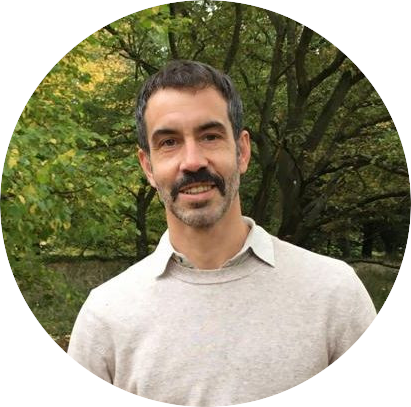
\includegraphics[width=3.5cm, right]{id-s}}

\includegraphics[scale=0.025]{gmail} \quad \href{mailto:thomas.huet@arch.ox.ac.uk}{thomas.huet@arch.ox.ac.uk} \& \href{mailto:thomashuet7@gmail.com}{thomashuet7@gmail.com}\\

\includegraphics[scale=0.010]{webpro} \quad \href{https://archit.web.ox.ac.uk/people/dr-thomas-huet}{School of Archaeology} \& \href{https://eamena.org/people/dr-thomas-huet}{projet EAMENA}\\

\includegraphics[scale=0.007]{lod-orcid} \quad \href{https://orcid.org/0000-0002-1112-6122}{0000-0002-1112-6122} \\

\includegraphics[scale=0.007]{github} \quad \href{https://github.com/zoometh/thomashuet.github.io/blob/main/README.md}{zoometh} \\

\includegraphics[scale=0.025]{gscholar} \quad \href{https://scholar.google.fr/citations?user=2hKEVaIAAAAJ}{2hKEVaIAAAAJ} \\

\includegraphics[scale=0.050]{rgate} \quad \href{https://www.researchgate.net/profile/Thomas\_Huet2}{Thomas\_Huet2} \\

\includegraphics[scale=0.005]{phone} \quad  \+ 44 (0)7 518 152 642 \\

%  example of 
% \title{\fr{Titre en Français}\en{Title in English}}

\section{\fr{SITUATION ACTUELLE (depuis 2021)}\en{CURRENT SITUATION (since 2021)}}
%\begin{itemize}
\textbf{Researcher and Database Manager}, University of Oxford, School of Archaeology, project 'Endangered Archaeology in the Middle East and North Africa' (EAMENA), 2 South Parks Road, Oxford OX1 3TG, United Kingdom.

\section{\fr{POSTES ACADÉMIQUES \textit{\&} PROFESSIONNELS (depuis 2013)}\en{ACADEMIC \textit{\&} PROFESSIONAL POSITIONS (since 2013)}}

\textbf{2021-7} 
\fr{Chercheur et responsable de la base de données EAMENA (\textit{Endangered Archaeology in the Middle East and North Africa}), Université d'Oxford, School of Archaeology, 2 South Parks Road, Oxford OX1 3TG, Royaume-Uni, novembre 2021-\\
\hspace*{0.5cm} Développement, administration et gestion de la base de données EAMENA, formation des utilisateurs et des gestionnaires des instances nationales, etc.}
\en{Researcher and Database Manager for EAMENA (\textit{Endangered Archaeology in the Middle East and North Africa}), University of Oxford, School of Archaeology, 2 South Parks Road, Oxford OX1 3TG, United Kingdom, November 2021-\\
\hspace*{0.5cm} Development, administration, and management of the EAMENA database, training of users and managers of national instances, etc.}

\smallbreak
\textbf{2021} 
\fr{Technicien de Support à la recherche (Técnico Especialista de Suport a la Recerca - TEC), Département de Préhistoire, Universitat Autònoma de Barcelona (UAB), Espagne, 1er juillet-31 octobre \\
\hspace*{0.5cm} Informatisation de la base de données des gravures médiévales de Sauri, développement de routines d'analyses (scripts R).}
\en{Research Support Technician (Técnico Especialista de Suport a la Recerca - TEC), Department of Prehistory, Universitat Autònoma de Barcelona (UAB), Spain, July 1 - October 31 \\
\hspace*{0.5cm} Computerization of the database of medieval engravings from Sauri, development of analysis routines (R scripts).}

\smallbreak
\textbf{2019-20} 
\fr{Chercheur Archaïos (compagnie privée), 1er juin - 1er juin \\
\hspace*{0.5cm} Chargé de l'intégration de la base de données et du SIG pour l'étude de l'oasis d'Al-'Ula (Arabie Saoudite).}
\en{Researcher at Archaïos (private company), June 1 - June 1 \\
\hspace*{0.5cm} Responsible for the integration of the database and GIS for the study of Al-'Ula oasis (Saudi Arabia).}
\smallbreak
\textbf{2019} 
\fr{Ingénieur d'études (IE), UMR 8546 CNRS/PSL-AOrOc, Paris et Allones, 1er juin - 1er juillet \\ 
\hspace*{0.5cm} Étude de faisabilité (prospection auprès des acteurs administratifs et de recherche, locaux, régionaux et nationaux) pour le redéploiement du Centre de Ressources Archéologique (CAPRA, Allones) en \textit{hub} technologique pour le service aux institutions de recherche en archéologie.}
\en{Study Engineer (IE), UMR 8546 CNRS/PSL-AOrOc, Paris and Allones, June 1 - July 1 \\ 
\hspace*{0.5cm} Feasibility study (outreach to local, regional, and national administrative and research stakeholders) for the redeployment of the Archaeological Resource Center (CAPRA, Allones) into a technological hub for service to archaeological research institutions.}
\smallbreak
\textbf{2018} \fr{Ingénieur de recherche (IR), UMR 7264 CEPAM-CNRS, Université Nice Sophia-Antipolis, projet \textit{Céramiques Imprimées de Méditerranée occidentale} (CIMO), 1er mai-30 août et 1er octobre-30 novembre} \en{Research Engineer, UMR 7264 CEPAM-CNRS, University of Nice Sophia-Antipolis, project \textit{Printed Ceramics of the Western Mediterranean} (CIMO), May 1-August 30 and October 1-November 30} \\
\hspace*{0.5cm} \fr{Modélisation des données archéologiques de la diffusion du Néolithique en Méditerranée centro-occidentale, routines d'analyses, développement de l'application web Leapfrog (scripts R)} \en{Modeling archaeological data on the spread of the Neolithic in the central-western Mediterranean, analysis routines, development of the Leapfrog web application (R scripts)}
\smallbreak
\textbf{--- } \fr{Ingénieur de recherche (IR), UMR 5140 ASM-CNRS, Université Paul Valéry Montpellier 3, projet \textit{EpiSpat} (aka \textit{ArchaEpigraph}), LabEx ARCHIMEDE, 1er avril-1er mai et 1er-30 septembre} \en{Research Engineer, UMR 5140 ASM-CNRS, Paul Valéry University Montpellier 3, project \textit{EpiSpat} (also known as \textit{ArchaEpigraph}), LabEx ARCHIMEDE, April 1-May 1 and September 1-30} \\
\hspace*{0.5cm} \fr{Étude statistiques et géostatistiques des stèles épigraphiques de la Narbonnaise antique, analyses à la volée de la base de données \textit{EpiSpat}(scripts R, connecteur ODBC, base de données FileMaker).} \en{Statistical and geostatistical studies of epigraphic steles from ancient Narbonnaise, on-the-fly analysis of the \textit{EpiSpat} database (R scripts, ODBC connector, FileMaker database).}

\smallbreak
\textbf{2015-6} \fr{Chercheur postdoctoral, LabEx ARCHIMEDE, UMR 5140 ASM-CNRS et Université Paul-Valéry, Montpellier. 1 octobre 2015 - 30 septembre 2016.} \en{Postdoctoral Researcher, LabEx ARCHIMEDE, UMR 5140 ASM-CNRS and University Paul-Valéry, Montpellier. October 1, 2015 - September 30, 2016.} \\
\hspace*{0.5cm} \fr{Étude des décors figuratifs en céramique de l'Âge du Bronze final dans le sud de la France et le nord-est de l'Espagne} \en{Study of figurative ceramic decorations from the Late Bronze Age in southern France and northeastern Spain}



\smallbreak
\textbf{2014} \fr{Ingénieur de recherche (IR), projet \textit{Archaepigraph}, UMR 6249 Chrono-Environnement, Université de Franche-Comté, 1er septembre-30 octobre} \en{Research Engineer, \textit{Archaepigraph} project, UMR 6249 Chrono-Environnement, University of Franche-Comté, September 1-October 30} \\
\hspace*{0.5cm} \fr{Étude statistiques, géostatistiques et de réseaux des stèles épigraphiques de la Narbonnaise antique.} \en{Statistical, geostatistical, and network studies of the epigraphic steles from ancient Narbonnaise.}
\smallbreak
\textbf{2013-4} \fr{Ingénieur d'études (IE), USR CNRS - UB 3516, plateforme GeoBFC, MSH de Dijon, Université de Bourgogne, projet OH-FET (Objet Historique, Fonction, Espace, Temps), 1er juin-31 mai} \en{Study Engineer, USR CNRS - UB 3516, GeoBFC platform, MSH of Dijon, University of Burgundy, OH-FET project (Historical Object, Function, Space, Time), June 1-May 31} \\
\hspace*{0.5cm} \fr{Développement de l'application OH-FET (Python) d'après le modèle conceptuel éponyme.} \en{Development of the OH-FET application (Python) based on the eponymous conceptual model.}




\section{\fr{PARCOURS ACADÉMIQUE}\en{ACADEMIC BACKGROUND}}

\textbf{2006-12} 
\fr{Doctorat en Histoire et Archéologie: "Organisation spatiale et sériation des gravures piquetées du mont Bego", mention très honorable avec les félicitations du jury, 29 mai 2012, Université Nice Sophia-Antipolis, UMR 7264 CEPAM-CNRS, HALtheses: \href{https://tel.archives-ouvertes.fr/tel-00712290}{tel-00712290}.}
\en{PhD in History and Archaeology: "Spatial Organization and Seriation of the Punched Engravings of Mount Bego", with high honors and jury's congratulations, May 29, 2012, University of Nice Sophia-Antipolis, UMR 7264 CEPAM-CNRS, HALtheses: \href{https://tel.archives-ouvertes.fr/tel-00712290}{tel-00712290}.}

\smallbreak
\textbf{2005-6} 
\fr{Master 2 Recherche en Histoire et Archéologie: "Étude des gravures protohistoriques de la zone des lacs (zones I, II, III et V) de la région du mont Bego, Tende, Alpes-Maritimes", mention bien, Université Nice Sophia-Antipolis, UMR 7264 CEPAM-CNRS, HALtheses: \href{https://tel.archives-ouvertes.fr/tel-00715386}{tel-00715386}.}
\en{Master of Research in History and Archaeology: "Study of Protohistoric Engravings in the Lake Area (zones I, II, III, and V) of Mount Bego, Tende, Alpes-Maritimes", with honors, University of Nice Sophia-Antipolis, UMR 7264 CEPAM-CNRS, HALtheses: \href{https://tel.archives-ouvertes.fr/tel-00715386}{tel-00715386}.}

\smallbreak
\textbf{2004-5} 
\fr{Diplôme universitaire de technologie (DUT) Génie informatique, Conservatoire National des Arts et Métiers (CNAM), Paris.}
\en{University Diploma in Technology (DUT) in Computer Engineering, Conservatoire National des Arts et Métiers (CNAM), Paris.}
% \smallbreak
% \textbf{2003} Diplôme de topographie, Universitad de Ingeniería, Lima, Pérou.
% \smallbreak
% \textbf{2002} Maîtrise en Archéologie (Master 1 Archéologie), Université Paris IV, Paris-Sorbonne, Paris.
% \smallbreak
% \textbf{2001} Licence en Archéologie, Université Paris IV, Paris-Sorbonne, Paris.
% \smallbreak
% \textbf{2000} DEUG Archéologie et Histoire de l'Art, Université Paris IV, Paris-Sorbonne, Paris.

\subsection*{\fr{Prix et récompenses}\en{Awards and Honors}}

\textbf{2024} 
\fr{Fonds John Fell (\textit{Social Science Division Fixed-Term Researchers Support Fund}) (£500).}
\en{John Fell Fund (\textit{Social Science Division Fixed-Term Researchers Support Fund}) (£500).}
\smallbreak
\textbf{--- } 
\fr{Fonds Meyerstein (£400).}
\en{Meyerstein Fund (£400).}
\smallbreak
\textbf{2023} 
\fr{Fonds Meyerstein (£400).}
\en{Meyerstein Fund (£400).}
\smallbreak
\textbf{2013} 
\fr{Prix de thèse pour publication. CASDEN-Banque Populaire (UFR LSH, Université Nice Sophia-Antipolis) (1500€).}
\en{Dissertation Prize for Publication. CASDEN-Banque Populaire (UFR LSH, University of Nice Sophia-Antipolis) (€1500).}

\section{\fr{PROJETS DE RECHERCHE \textit{\&} ACADÉMIQUES (depuis 2014)}\en{RESEARCH \textit{\&} ACADEMIC PROJECTS (since 2014)}}

\textbf{2022}
\fr{Chercheur invité, \textit{Dipartimento di Civiltà e forme del Sapere}, Università di Pisa, 11 mars - 15 avril (1 mois).}
\en{Visiting Researcher, \textit{Department of Civilisations and Forms of Knowledge}, University of Pisa, March 11 - April 15 (1 month).}

\smallbreak

\subsection*{\fr{Programmes de recherche (Membre depuis)}\en{Research Programs (Member since)}}
\subsubsection*{\fr{En cours}\en{Research Programs (Ongoing)}}

\textbf{2024 }
\fr{I+D "Advances in computational simulation of the Neolithic spread in Europe: integrating archaeological and ancient genetic data", 2024-2027, PI: Joaquim Fort Viader, Universitat de Girona, Espagne}
\en{I+D "Advances in computational simulation of the Neolithic spread in Europe: integrating archaeological and ancient genetic data", 2024-2027, PI: Joaquim Fort Viader, University of Girona, Spain}

\textbf{2024 }
\fr{I+D "Identification of domestic units and domestic production through multifactorial analysis in the Western Catalan Plain between the 4th and 1st millennium BCE (HOUSEPROD)", 2024-2027, PI: Natàlia Alonso Martínez et Georgina Prats Ferrando, Universitat de Lleida, Spain}
\en{I+D "Identification of domestic units and domestic production through multifactorial analysis in the Western Catalan Plain between the 4th and 1st millennium BCE (HOUSEPROD)", 2024-2027, PI: Natàlia Alonso Martínez and Georgina Prats Ferrando, University of Lleida, Spain}

\textbf{2022 }
\fr{I+D "Equid introduction, hybridisation and agricultural intensification in the Ebro valley from the Late Neolithic to the Iron Age (CENTAURO)", 2022-2025, PI: Ariadna Nieto-Espinet, University of Lleida, Spain (2022-2025) \href{https://www.centaur-o.com/}{
\includegraphics[scale=0.015]{link_darkblue.png}}}
\en{I+D "Equid introduction, hybridisation and agricultural intensification in the Ebro valley from the Late Neolithic to the Iron Age (CENTAURO)", 2022-2025, PI: Ariadna Nieto-Espinet, University of Lleida, Spain (2022-2025), \href{https://www.centaur-o.com/}{
\includegraphics[scale=0.015]{link_darkblue.png}}}

% \textbf{2021 }
% \fr{Comité de gestion du projet EAMENA \href{https://eamena.org/}{
\includegraphics[scale=0.015]{link_darkblue.png}}}
% \en{EAMENA Project Management Committee \href{https://eamena.org/}{
\includegraphics[scale=0.015]{link_darkblue.png}}}

\textbf{2021}
\fr{ANR Italic metalwork Techniques during the Early Iron AgE (Itineris) - Agence Nationale pour la Recherche, PI: Veronica Ciccolani, CNRS, France (2021-2024) \href{https://anr.fr/Project-ANR-21-CE27-0010}{
\includegraphics[scale=0.015]{link_darkblue.png}}}
\en{ANR Italic metalwork Techniques during the Early Iron AgE (Itineris) - National Research Agency, PI: Veronica Ciccolani, CNRS, France (2021-2024) \href{https://anr.fr/Project-ANR-21-CE27-0010}{
\includegraphics[scale=0.015]{link_darkblue.png}}}


% \subsubsection*{\fr{Groupes de travail}\en{Working groups}}
% \textbf{2020}
% \fr{Projet collectif de recherche \textit{NeoNet}(2020-...) \href{https://redneonet.com/}{
\includegraphics[scale=0.015]{link_darkblue.png}}}
% \en{NeoNet Research Collective Project (2020-...) \href{https://redneonet.com/}{
\includegraphics[scale=0.015]{link_darkblue.png}}}
% \smallbreak
% \textbf{2020}
% \fr{Groupe d'intérêt spécial sur les langages de script scientifiques en archéologie (\textit{Special Interest Group on Scientific Scripting Languages in Archaeology}, SIG-SSLA) \href{https://sslarch.github.io/}{
\includegraphics[scale=0.015]{link_darkblue.png}}}
% \en{Special Interest Group on Scientific Scripting Languages in Archaeology (SIG-SSLA) \href{https://sslarch.github.io/}{
\includegraphics[scale=0.015]{link_darkblue.png}}}
% \smallbreak
% \textbf{2020}
% \fr{Groupe d'archéologie de haute montagne (\textit{Grup d'Arqueologia de l'Alta Muntanya}, GAAM), Universitat Autònoma de Barcelona et Consejo Superior de Investigaciones Cientificas (UAB-CSIC) \href{https://arqueologiademuntanya.wordpress.com/}{
\includegraphics[scale=0.015]{link_darkblue.png}}}
% \en{High Mountain Archaeology Group (\textit{Grup d'Arqueologia de l'Alta Muntanya}, GAAM), Autonomous University of Barcelona and Spanish National Research Council (UAB-CSIC) \href{https://arqueologiademuntanya.wordpress.com/}{
\includegraphics[scale=0.015]{link_darkblue.png}}}

\subsection*{\fr{Responsabilités académiques (depuis 2023)}\en{Academic Responsibilities (since 2023)}}

\textbf{2023}
\fr{Représentant des chercheurs (niveau Université) - Groupe de pilotage sur le libre accès (\textit{Open Access Steering Group}, OASG), Université d'Oxford (2023-...) \href{https://researchsupport.admin.ox.ac.uk/oasg}{
\includegraphics[scale=0.015]{link_darkblue.png}}}
\en{Researcher Representative (University Level) - Open Access Steering Group (OASG), University of Oxford (2023-...) \href{https://researchsupport.admin.ox.ac.uk/oasg}{
\includegraphics[scale=0.015]{link_darkblue.png}}}

\textbf{2023}
\fr{Trésorier - Société pour le personnel enseignant et de recherche postdoctoral et en début de carrière en archéologie (\textit{Society for Postdoctoral and Early Career Teaching and Research Staff in Archaeology}, SPECTRA) \href{https://spectra.arch.ox.ac.uk/}{
\includegraphics[scale=0.015]{link_darkblue.png}}}
\en{Treasurer - Society for Postdoctoral and Early Career Teaching and Research Staff in Archaeology (SPECTRA) \href{https://spectra.arch.ox.ac.uk/}{
\includegraphics[scale=0.015]{link_darkblue.png}}}

\textbf{2023}
\fr{Expert - Agence Nationale pour la Recherche (ANR) \href{https://iris.anr.fr/}{
\includegraphics[scale=0.015]{link_darkblue.png}}}
\en{Expert - French National Research Agency (ANR) \href{https://iris.anr.fr/}{
\includegraphics[scale=0.015]{link_darkblue.png}}}

\smallbreak

\subsection*{\fr{Comités de revues scientifiques (depuis 2014)}\en{Scientific Review Committees (since 2014)}}

\textbf{2021}
\fr{Membre du comité éditorial de \textit{Préhistoires Méditerranéennes} journal}
\en{Editorial Committee Member of \textit{Préhistoires Méditerranéennes} journal}

\textbf{2023}
\fr{Recommandeur et Relecteur pour \textit{PCI Archaeology} \href{https://archaeo.peercommunityin.org/public/user_public_page?userId=1235}{
\includegraphics[scale=0.02]{link_grey.png}}}
\en{Recommender and Reviewer for \textit{PCI Archaeology} \href{https://archaeo.peercommunityin.org/public/user_public_page?userId=1235}{
\includegraphics[scale=0.02]{link_grey.png}}}


\textbf{-}
\fr{\textbf{Relecteur} pour: \textit{ArcheoLogica-Data} journal (2022-...), \textit{Journal of Open Source Software} (2021-...), \textit{Journal of Computer Applications for Archaeology} (2021-...) et \textit{CAA Review College} (2014-...), \textit{Bulletin de la Société Préhistorique Française} journal (2020-...), \textit{M@ppemonde} journal (2019-...)}
\en{\textbf{Reviewer} for: \textit{ArcheoLogica-Data} journal (2022-...), \textit{Journal of Open Source Software} (2021-...), \textit{Journal of Computer Applications for Archaeology} (2021-...) and \textit{CAA Review College} (2014-...), \textit{Bulletin de la Société Préhistorique Française} journal (2020-...), \textit{M@ppemonde} journal (2019-...)}

\section*{\fr{ENSEIGNEMENTS, FORMATIONS \textit{\&} ENCADREMENTS DISPENSÉS}\en{TEACHING, TRAINING \textit{\&} SUPERVISION ACTIVITIES}}

\subsection*{\fr{Enseignements et Formations dispensées}\en{Teaching and Training activities}}

\textbf{2024}
\fr{"EAMENA database", \textit{Endangered Archaeology in the Middle East and North Africa} (EAMENA) project, \textit{British Council Cultural Protection Fund} (CPF) \textit{training}, General Directorate of Antiquities and Heritage (GDAH), Kurdistan Region Iraq, 2-7 Mars (3 jours).}
\en{"EAMENA database", \textit{Endangered Archaeology in the Middle East and North Africa} (EAMENA) project, \textit{British Council Cultural Protection Fund} (CPF) \textit{training}, General Directorate of Antiquities and Heritage (GDAH), Kurdistan Region Iraq, March 2-7 (3 days).}

\smallbreak
\textbf{--- }
\fr{"Authoring, writing and publishing with R Markdown", Winter School 'R 4 Archeologists', \textit{Progetto metodologie applicate all predittivita del potenziale archeologico} (mappa), Università di Pisa, 2 Janvier (3 heures), \href{https://github.com/zoometh/thomashuet/tree/main/teach/stats/r4a}{
\includegraphics[scale=0.015]{link_darkblue.png}}.}
\en{"Authoring, Writing and Publishing with R Markdown", Winter School 'R 4 Archaeologists', \textit{Project on Applied Methodologies for Predictive Archaeological Potential} (mappa), University of Pisa, January 2 (3 hours), \href{https://github.com/zoometh/thomashuet/tree/main/teach/stats/r4a}{
\includegraphics[scale=0.015]{link_darkblue.png}}.}

\smallbreak
\textbf{2023}
\fr{"Why R ?", Workshop R, School of Archaeology, Oxford, 5 Décembre.}
\en{"Why R?", R Workshop, School of Archaeology, Oxford, December 5.}

\smallbreak
\textbf{--- }
\fr{"EAMENA database", \textit{Endangered Archaeology in the Middle East and North Africa} (EAMENA) project, \textit{British Council Cultural Protection Fund} (CPF) \textit{training}, Amman, Jordan, 18-22 Juin (4 jours).}
\en{"EAMENA Database", \textit{Endangered Archaeology in the Middle East and North Africa} (EAMENA) project, \textit{British Council Cultural Protection Fund} (CPF) \textit{training}, Amman, Jordan, June 18-22 (4 days).}

\smallbreak
\textbf{--- }
\fr{"Initiation aux statistiques", MASTER parcours Géo-bioarchéo, \textit{TW223AH Atelier traitement des données}, Université de Montpellier, 20-22 Février (6 heures), \href{http://shinyserver.cfs.unipi.it:3838/teach/stats/upv/_site/#/title-slide}{
\includegraphics[scale=0.015]{link_darkblue.png}}.}
\en{"Introduction to Statistics", MASTER in Geo-bioarchaeology, \textit{TW223AH Data Processing Workshop}, University of Montpellier, February 20-22 (6 hours), \href{http://shinyserver.cfs.unipi.it:3838/teach/stats/upv/_site/#/title-slide}{
\includegraphics[scale=0.015]{link_darkblue.png}}.}

\smallbreak
\textbf{--- }
\fr{"Report with R Markdown", Winter School 'R 4 Archeologists', \textit{Progetto metodologie applicate all predittivita del potenziale archeologico} (mappa), Università di Pisa, 8 Février (3 heures), \href{https://github.com/zoometh/thomashuet/tree/main/teach/stats/r4a}{
\includegraphics[scale=0.015]{link_darkblue.png}}.}
\en{"Report with R Markdown", Winter School 'R 4 Archaeologists', \textit{Project on Applied Methodologies for Predictive Archaeological Potential} (mappa), University of Pisa, February 8 (3 hours), \href{https://github.com/zoometh/thomashuet/tree/main/teach/stats/r4a}{
\includegraphics[scale=0.015]{link_darkblue.png}}.}

\smallbreak
\textbf{--- }
\fr{"Arches/EAMENA Database Manager training (part 2/2)", \textit{Endangered Archaeology in the Middle East and North Africa} (EAMENA) project, \textit{British Council Cultural Protection Fund} (CPF) \textit{training}, University of Oxford, 14-16 Février (9 heures), \href{https://github.com/eamena-oxford/eamena-arches-dev/tree/main/training#readme}{
\includegraphics[scale=0.015]{link_darkblue.png}}.}
\en{"Arches/EAMENA Database Manager Training (part 2/2)", \textit{Endangered Archaeology in the Middle East and North Africa} (EAMENA) project, \textit{British Council Cultural Protection Fund} (CPF) \textit{training}, University of Oxford, February 14-16 (9 hours), \href{https://github.com/eamena-oxford/eamena-arches-dev/tree/main/training#readme}{
\includegraphics[scale=0.015]{link_darkblue.png}}.}

\smallbreak
\textbf{2021}
\fr{"Arches/EAMENA Database Manager training (part 1/2)", \textit{Endangered Archaeology in the Middle East and North Africa} (EAMENA) project, \textit{British Council Cultural Protection Fund} (CPF) \textit{training}, Amman, 5 - 9 Décembre (5 jours), \href{https://github.com/eamena-oxford/eamena-arches-dev/tree/main/training#readme}{
\includegraphics[scale=0.015]{link_darkblue.png}}.}
\en{"Arches/EAMENA Database Manager Training (part 1/2)", \textit{Endangered Archaeology in the Middle East and North Africa} (EAMENA) project, \textit{British Council Cultural Protection Fund} (CPF) \textit{training}, Amman, December 5 - 9 (5 days), \href{https://github.com/eamena-oxford/eamena-arches-dev/tree/main/training#readme}{
\includegraphics[scale=0.015]{link_darkblue.png}}.}

\smallbreak
\textbf{2017}
\fr{"Introduction to Geographic Information Systems: QGIS", \textit{Grupo de Arqueologia de las Dinámicas Sociales}, Consejo Superior de Investigaciones Cientificas, Institución Milá i Fontanals (CSIC-IMF), 14-16 Décembre (9 heures).}
\en{"Introduction to Geographic Information Systems: QGIS", \textit{Group of Archaeology of Social Dynamics}, Spanish National Research Council, Institución Milá i Fontanals (CSIC-IMF), December 14-16 (9 hours).}

\smallbreak
\textbf{2016}
\fr{"Méthodes quantitatives en archéologie. L'approche processuelle : concepts, outils et cas d'étude" Master 2 Archéologie, Sciences pour l'Archéologie, ASM-UMR 5140, University seminar, Université Paul-Valéry, 5 Décembre (4 heures).}
\en{"Quantitative Methods in Archaeology. The Processual Approach: Concepts, Tools, and Case Studies" Master 2 in Archaeology, Sciences for Archaeology, ASM-UMR 5140, University Seminar, Paul-Valéry University, December 5 (4 hours).}

\smallbreak
\textbf{2015}
\fr{"L'apparition des décors figuratifs du Mailhac I et des groupes apparentés dans une Europe continentale largement aniconique (Bronze final IIIb, 950-750 av. J.-C.) : contextes, hypothèses et méthodes" Master 1 Recherche, Protohistoire méditerranéenne, ACTE -- UE 3-6, University seminar, Université de Bourgogne, 24 Novembre (1 heure).}
\en{"The Emergence of Figurative Decorations from Mailhac I and Related Groups in a Predominantly Aniconic Continental Europe (Late Bronze Age IIIb, 950-750 BC): Contexts, Hypotheses, and Methods" Master 1 Research, Mediterranean Protohistory, ACTE -- UE 3-6, University Seminar, University of Burgundy, November 24 (1 hour).}

\smallbreak
\textbf{--- }
\fr{"L'apport du SIG à l'étude de l'art rupestre du Mont Bego (Alpes-Maritimes)" Master 2 Recherche et Professionnel, Archéologie des Sociétés et Territoires en France Métropolitaine, Méthodes et approches nouvelles, LARA, CReAAH-UMR 6566, University seminar, Université de Nantes, Université de Rennes, 4 Novembre (1 heure).}
\en{"The Contribution of GIS to the Study of Rock Art at Mont Bego (Alpes-Maritimes)" Master 2 Research and Professional, Archaeology of Societies and Territories in Metropolitan France, New Methods and Approaches, LARA, CReAAH-UMR 6566, University Seminar, University of Nantes, University of Rennes, November 4 (1 hour).}

\smallbreak
\textbf{--- }
\fr{"Les méthodes quantitatives en archéologie : de la \textit{New Archaeology} au \textit{Project Mosul}" Master 2 Recherche et Professionnel, Archéologie des Sociétés et Territoires en France Métropolitaine, Séminaire spécialisé : "Méthodes et approches nouvelles", LARA, CReAAH-UMR 6566, University seminar, Université de Nantes, Université de Rennes, 16 Octobre (1 heure).}
\en{"Quantitative Methods in Archaeology: From \textit{New Archaeology} to \textit{Project Mosul}" Master 2 Research and Professional, Archaeology of Societies and Territories in Metropolitan France, Specialized Seminar: "New Methods and Approaches", LARA, CReAAH-UMR 6566, University Seminar, University of Nantes, University of Rennes, October 16 (1 hour).}

\smallbreak
\textbf{2013}
\fr{"Systèmes symboliques", ETD Master 1 Préhistoire, Paléoenvironnement et Archéosciences (SMZTPP16), Université Nice Sophia-Antipolis (3 heures).}
\en{"Symbolic Systems", ETD Master 1 in Prehistory, Paleoenvironment, and Archaeosciences (SMZTPP16), University of Nice Sophia-Antipolis (3 hours).}

\subsection*{\fr{Encadrements}\en{Supervisions}}

\textbf{2015-23}
\fr{Membre du comité de suivi de la thèse de Francis Bordas, Université Toulouse 2, École doctorale TESC, UMR TRACES. Titre de la thèse : "Les dépôts métalliques du BFa 3 (950-800 av. J.-C.) en Gaule atlantique Modalités de circulation, de manipulation et d’enfouissement du métal".}
\en{Member of the thesis monitoring committee for Francis Bordas, University of Toulouse 2, Doctoral School TESC, UMR TRACES. Thesis title: "Metallic deposits of BFa 3 (950-800 BC) in Atlantic Gaul: Modes of circulation, handling, and burial of metal".}

\smallbreak
\textbf{2018-9}
\fr{Tuteur du Master 2 de Marco Padovan, Università degli Studi di Ferrara, Corso di Laurea Magistrale in Quaternario, Preistoria e Archeologia. "Analyse de la céramique des couches mésolithiques à Baume du Monthiver (Comps-sur-Artuby, Var, France)".}
\en{Supervisor for the Master 2 of Marco Padovan, University of Ferrara, Master's Degree in Quaternary, Prehistory and Archaeology. "Analysis of the ceramics from the Mesolithic layers at Baume du Monthiver (Comps-sur-Artuby, Var, France)".}

\section{PUBLICATIONS}

\subsection*{\fr{Articles}\en{Articles}}
$\bullet$ Ciccolani V. et \textbf{Huet T.}, (\textbf{2024}). Modélisation exploratoire des interactions entre entités culturelles en Italie du Nord au premier âge du Fer : entre centres et périphéries, \textit{Bulletin de la Soci\'{e}t\'{e} Pr\'{e}historique Fran\c{c}aise}.
\smallbreak
$\bullet$ Rouhani B. et \textbf{Huet T.}, (\textbf{2024}). Historical Landscape of Sistan in Iran and Afghanistan: EAMENA Dataset for Assessing Environmental Impact on Cultural Heritage, \textit{Journal of Open Archaeology Data}, DOI: \href{https://openarchaeologydata.metajnl.com/articles/10.5334/joad.123}{10.5334/joad.123}.
\smallbreak
$\bullet$ \textbf{Huet T.}, Basílio MA.C., Carvalho A.F., Cubas M., Gibaja J.F, López-Romero E., Oms F.X. et N. Mazzucco (\textbf{2024}). NeoNet Atlantic. Radiocarbon Dates for the Late Mesolithic/Early Neolithic Transition in the Southern European Atlantic Coast, \textit{Journal of Open Archaeology Data}, DOI: \href{https://openarchaeologydata.metajnl.com/articles/10.5334/joad.120}{10.5334/joad.120}.
\smallbreak
$\bullet$ Charbonnier J., Kanhoush Y., Gravier J., Gourret G., Achouche I., Bernollin V., Boudia S., Bucci W., Chiti B., Clauss-Balty P., Colard V., Devaux E., Dupont-Delaleuf A., De Smet A., Furstos C., Goy J., Haze M., Hofstetter T., Housse R., \textbf{Huet T.}, Marquaire C., Paola Pellegrino M., Raad C., Ricart J.-D., Rosak A., Said A.F., Serres D., Simeon P., Tourtet F. et J. Giraud (\textbf{2023}). Mapping an Arabian oasis: first results of UCOP systematic survey of al-'Ula Valley (2019-2021), \textit{Proceedings of the Seminar for Arabian Studies (PSAS)}
\smallbreak
$\bullet$ \textbf{Huet T.}, Cubas M., Gibaja J.F., Oms F.X. and N. Mazzucco (\textbf{2022}). NeoNet Dataset. Radiocarbon Dates for the Late Mesolithic/Early Neolithic Transition in the North Central-Western Mediterranean Basin, \textit{Journal of Open Archaeology Data}, DOI: \href{http://doi.org/10.5334/joad.87}{10.5334/joad.87}.
\smallbreak
$\bullet$ \textbf{Huet T.}, Pozo J. M. et Alexander C. (\textbf{2021}), Analysis of Prehistoric Iconography with the R package \textit{iconR}, \textit{Journal of Open Statistical Software}, \href{https://joss.theoj.org/papers/10.21105/joss.03191}{10.21105/joss.03191}.
\smallbreak
$\bullet$ Nieto-Espinet A., \textbf{Huet T.}, Trentacoste A., Guimaraes S., Orengo H. and S. Valenzuela-Lamas (\textbf{2021}). Resilience and livestock adaptations to demographic growth and technological change: A diachronic perspective from the Late Bronze Age to Late Antiquity in NE Iberia, \textit{PlosONE}, DOI: \href{https://doi.org/10.1371/journal.pone.0246201}{10.1371/journal.pone.0246201}
\smallbreak
$\bullet$ Iba\~{n}ez J.J., Mu\~{n}iz J., \textbf{Huet T.}, Borrell Terra F.,.Santana Y., Teira Mayolini L.C. and R. Rosillo (\textbf{2020}). Flint Figurines in the Early Neolithic site of Kharaysin (Early 8th Millennium BC, Jordan), \textit{Antiquity Journal, 94, 376}, 880-899, DOI: \href{https://doi.org/10.15184/aqy.2020.78}{10.15184/aqy.2020.78}.
\smallbreak
$\bullet$ Cicolani V. et \textbf{T. Huet} (\textbf{2019}). Essai de mod\'{e}lisation des \'{e}changes et des r\'{e}seaux de circulation dans les Alpes centrales au premier \^{a}ge du Fer, \textit{in} Deschamps M., Costamagno S., Milcent P.-Y., Pétillon J.-M., Renard C. and N. Valdeyron (dir.) "La conqu\^{e}te de la montagne : des premi\'{e}res occupations humaines \`{a} l'anthropisation du milieu", \textit{Comit\'{e} des Travaux Historiques et Scientifiques \'{e}ditions} (CTHS), DOI: \href{https://books.openedition.org/cths/7827}{10.4000/books.cths.7827}.
\smallbreak
$\bullet$ \textbf{Huet T.} (\textbf{2018}). Geometric Graphs to Study Ceramic Decoration, \textit{in} M. Matsumoto and.E. Uleberg (eds), Exploring Oceans of Data, \textit{Proceedings of the 44${}^{nd\ }$Conference on Computer Applications and quantitative Methods in Archaeology} (CAA2016), Oxford : Archaeopress Archaeology, 311-323, HAL: \href{https://hal.archives-ouvertes.fr/hal-02913656}{hal-02913656}
\smallbreak
$\bullet$ \textbf{Huet T.} (\textbf{2016}). New perspectives on the chronology and the meaning of Mont Bego's rock-art (Alpes-Maritimes, France), \textit{Cambridge Archaeological Journal} 41, 1-23, DOI: \href{https://doi.org/10.1017/s0959774316000524}{10.1017/s0959774316000524}.
\smallbreak
$\bullet$ \textbf{Huet T.} et N. Bianchi (\textbf{2016}). Reticolati, pelli e mappe topografiche, lo stato della ricerca al monte Bego, \textit{Bollettino del Centro Camuno di Studi Preistorici} 41, 31-43, ISSN 1594-7084 \href{http://www.ccsp.it/web/infoccsp/bcsp/bcsp41_preview.pdf}{
\includegraphics[scale=0.015]{link_darkblue.png}}.
\smallbreak
$\bullet$ \textbf{Huet T.} et N. Bianchi (\textbf{2016}). A study of the Roche de l'Autel's pecked engravings, Les Merveilles sector, Mont Bego area (Alpes-Maritimes, France), \textit{Journal of Archaeological Sciences: Reports} 5, 105-118, DOI: \href{https://doi.org/10.1016/j.jasrep.2015.11.006}{10.1016/j.jasrep.2015.11.006}.
\smallbreak
$\bullet$ \textbf{Huet T.} (\textbf{2016}). S\'{e}riation des gravures piquet\'{e}es du mont Bego, \textit{Archeologia e Calcolatori} 27, 65-83, DOI: \href{https://doi.org/10.19282/AC.27.2016.02}{10.19282/AC.27.2016.02}.
\smallbreak
$\bullet$ \textbf{Huet T.} (\textbf{2015}). Le incisioni a martellina del monte Bego: approcci geografici e quantitativi, \textit{Archeologia Postmedievale} 17, 329-338, ISSN 1592-5935 \href{https://www.insegnadelgiglio.it/wp-content/uploads/2015/01/APM_17_libro-anteprima.pdf}{
\includegraphics[scale=0.015]{link_darkblue.png}}.
\smallbreak
$\bullet$ Saligny L., Granjon L., \textbf{Huet T.}, Simon G., Rodier X. et B. Lefebvre (\textbf{2015}). OH\_FET: A Computer Application for Analysing Urban Dynamics Over Long Time Spans, in Giligny F., Djindjian F., Costa L., Moscati P. et S. Robert (eds) \textit{Proceedings of the 42${}^{nd\ }$Conference on Computer Applications and quantitative Methods in Archaeology} (CAA2014), Oxford : Archaeopress Archaeology, 381-392, HAL: \href{https://hal.archives-ouvertes.fr/halshs-01146871}{halshs-01146871}.
\smallbreak
$\bullet$ \textbf{Huet T.} et C. Alexander (\textbf{2015}). M\'{e}thodes informatiques pour l'\'{e}tude des gravures rupestres~: les exemples du Valcamonica (Italie) et du mont Bego (France), in Cervel M., Rousseau L. et M. Nordez (eds) \textit{Recherches sur l'\^{a}ge du Bronze. Nouvelles approches et perspectives. Actes de la journ\'{e}e d'\'{e}tude de l'APRAB, Bulletin de l'APRAB, suppl. 1}, 15-29 
\href{https://www.researchgate.net/publication/347437308_Methodes_informatiques_pour_l'etude_des_gravures_rupestres_les_exemples_du_Valcamonica_Italie_et_du_mont_Bego_France}{
\includegraphics[scale=0.015]{link_darkblue.png}}.
\smallbreak
$\bullet$ Ouriachi M.-J., Favory F., Garmy P., Ouzoulias P., Pasqualini A., Christol M., \textbf{Huet T}., Nuninger L., Bertoncello F. et R. H\"{a}ussler (\textbf{2014}). ArchaEpigraph : l'\'{e}pigraphie spatiale au service de l'\'{e}tude des dynamiques des territoires, in \textit{Revue arch\'{e}ologique de Narbonnaise}, tome 47, pp. 35-49, DOI: \href{https://doi.org/10.3406/ran.2014.1897}{10.3406/ran.2014.1897}.
\smallbreak
$\bullet$ \textbf{Huet T.} (\textbf{2014}). Use of quantitative methods to study an Alpine rock art site: the Mont Bego region, in Earl G., Sly T., Chrysanthi A., Murrieta Flores P., Papadopoulos C., Romanowska I. et D. Wheatley (eds) \textit{Proceedings of the 40${}^{th}$ Conference on Computer Applications and quantitative Methods in Archaeology} (CAA2012), Southampton, UK, 26-30 March 2012, Amsterdam : Pallas Publications, 584-591.
\smallbreak
$\bullet$ \textbf{Huet T.} (\textbf{2014}). Organisation spatiale et s\'{e}riation des gravures piquet\'{e}es du mont Bego~-- R\'{e}sum\'{e} de th\'{e}se, \textit{Bulletin de la Soci\'{e}t\'{e} Pr\'{e}historique Fran\c{c}aise} 110, 146-148, \href{https://www.persee.fr/doc/bspf_0249-7638_2013_num_110_1_14242}{
\includegraphics[scale=0.015]{link_darkblue.png}}.

% \subsubsection*{\fr{\begin{center}------------ Soumis/Accepté ------------\end{center}}\en{{\begin{center}------------ Submitted/Accepted ------------\end{center}}}}
\smallbreak
\fr{\begin{center}------------ Soumis/Accepté ------------\end{center}}\en{{\begin{center}------------ Submitted/Accepted ------------\end{center}}}
\smallbreak
$\bullet$ Nieto-Espinet A., Trentacoste A. , Cardona G., Carrocio M.,  Bòria A., \textbf{Huet T.}, Guimarães S., Pena L., García-Solsona E., Torner-Pérez J. et  Valenzuela-Lamas S. (\textit{\textbf{accepté}}). Estudi pioner en la detecció de la mobilitat estacional moderna mitjançant l'anàlisi d'isòtops estables d'estronci i oxigen. Un exemple d'investigació col·laborativa i lenta amb ramaders en extensiu dels Pirineus de Lleida. In Trepat, E., Borrell, M., Nieto-Espinet, A., Villalba, D. (eds). \textit{Actes del 2on Congrés de Transhumància i Camins Ramaders de Catalunya}, IDAPA (Institut per al Desenvolupament de Pirineu i Aran), Lleida. 
\smallbreak
$\bullet$ Gassiot Ballbè E., Augé Martínez O., Lapedra Grau S., \textbf{Huet T.}, Sánchez Bonastre X. et R. Martí Castelló (\textit{\textbf{soumis}}). Paisatges de conflicte i poder. Els gravats medievals del Solà de Saurí, (Pallars Sobirà), \textit{Tribuna d'Arqueologia}
\smallbreak
$\bullet$ Cicolani V., \textbf{Huet T.} et L. Zamboni (\textit{\textbf{soumis}}). Centre et marges, une approche critique : modélisation des interactions entre entités culturelles en Italie du Nord à l'âge du Fer, \textit{Comit\'{e} des Travaux Historiques et Scientifiques \'{e}ditions} (CTHS)
\smallbreak
$\bullet$ Pasqualini A., \textbf{Huet T.} et M.-J. Ouriachi (\textit{\textbf{soumis}}). Une base de données informatique dédiée au programme Epispat, \textit{in} Ouriachi M.-J. et Pellecuer C. (eds), \textit{Actes de la Table-ronde de cl\^{o}ture du programme Epispat, 21-22 nov. 2019, Hi\'{e}rarchie sociale et d\'{e}veloppement territorial en Gaule Narbonnaise et dans les provinces voisines : enqu\^{e}tes au croisement de l'\'{e}pigraphie et de l'arch\'{e}ologie spatiale}, Revue Arch\'{e}ologique de Narbonnaise.
\smallbreak

\subsection*{\fr{Ouvrages}\en{Books}}

\smallbreak
$\bullet$ \textbf{Huet T.} (\textbf{2017}). \textit{Les gravures piquet\'{e}es du mont Bego (Alpes-Maritimes). Organisation spatiale et s\'{e}riation (6e -- 2e mill\'{e}naire av. J.-C.)}, M\'{e}moire de la Soci\'{e}t\'{e} Pr\'{e}historique Fran\c{c}aise (SPF) 63, 166 p., ISBN : 2-913745-71-7 \href{http://www.prehistoire.org/shop_515-40342-0-0/m63-2017-les-gravures-piquetees-du-mont-bego-alpes-maritimes-organisation-spatiale-et-seriation-vie-iie-millenaire-av.-j.-c.-t.-huet.html}{
\includegraphics[scale=0.015]{link_darkblue.png}}

\bigbreak

\subsection*{\fr{Ouvrages (chapitres d')}\en{Book Chapters}}

$\bullet$ Binder D., Gomart L., \textbf{Huet T.}, Ka{\v{c}}ar S., Maggi R., Manen C., Radi G., et Tozzi C. avec la collaboration de Mutoni I.M., Natali E. et C. Panelli (\textbf{2022}). Le complexe de la C\'{e}ramique imprim\'{e}e de M\'{e}diterran\'{e}e centrale et occidentale : une synthèse chrono-culturelle (7e et 6e millénaires BCE), in Binder D. and C. Manen (dir), \textit{C\'{e}ramiques imprim\'{e}es de M\'{e}diterran\'{e}e occidentale (6e mill\'{e}naire BCE) : Donn\'{e}es, approches et enjeux nouveaux. Actes des journ\'{e}es de la Soci\'{e}t\'{e} Pr\'{e}historique Fran\c{c}aise, Nice, 18-20 mars 2019}, Paris: Soci\'{e}t\'{e} Pr\'{e}historique Fran\c{c}aise, p. 27-104, ISSN: 2263-3847, SPF: \href{https://www.prehistoire.org/515_p_57657/accEs-libre-seance-18-ceramiques-imprimees-de-mediterranee-occidentale.html}{spf-515}
\smallbreak
$\bullet$ Lanaspa J. R., Conte I. C., Gassiot Ballbè E., Mazzucco N., \textbf{Huet T.}, Olomi A. et J. Borràs (\textbf{2022}). Artiga Viturián, un nuevo yacimiento del Neolítico Antiguo en Sobrarbe (Huesca) in IV Congreso CAPA, Arqueología Patrimonio Aragonés, 29–36, ISBN: 978-84-09-41553-3.
\smallbreak
$\bullet$ Alexander C., Maretta A., \textbf{Huet T.} et C. Chippindale (\textbf{2021}). Rules of ordering and grouping in the 'pitoti', the later prehistoric rock-engravings of Valcamonica (BS), Italy: from solitary figures through clusters, graphic groups, and scenes to narrative, in I. Davidson and A. Nowell (eds), \textit{Making scenes: global perspectives on scenes in rock art}, London: Berghahn Books, p. 259-276 \href{https://www.berghahnbooks.com/title/DavidsonMaking}{
\includegraphics[scale=0.015]{link_darkblue.png}}.
\smallbreak
$\bullet$ \textbf{Huet T.} (\textbf{2018}). Une revue de l'iconographie du d\'{e}but du N\'{e}olithique \`{a} la fin de l'\^{a}ge du Bronze (ca. 5700-750 av. J.-C.) en France, \textit{in} Guilaine J. et D. Garcia (dir.), \textit{La Protohistoire de la France}, ed. Hermann, Paris, p. 221-249, HAL: \href{https://hal.archives-ouvertes.fr/hal-01983284}{hal-01983284}.
\smallbreak
\fr{\begin{center}------------ Soumis/Accepté ------------\end{center}}\en{{\begin{center}------------ Submitted/Accepted ------------\end{center}}}
\smallbreak
$\bullet$ \textbf{Huet T.} et N. Bianchi (\textbf{accepté}). Le Mont Bégo, in Marcigny C. et Mordant C. (eds), \textit{L'âge du Bronze en France}, Paris: Inrap / Presses du CNRS

\bigbreak

\subsection*{\fr{Conférences scientifiques et séminaires (2014-)}\en{Scientific Conferences and Seminars (2014-)}}

\begin{center}
\fr{(\textbf{i}) Audience internationale {\textbar} (\textbf{n}) Audience nationale}
\en{(\textbf{i}) International Audience {\textbar} (\textbf{n}) National Audience}
\end{center}

\smallbreak

\begin{center}
\fr{------------ Organisation ------------}
\en{------------ Organization ------------}
\end{center}

\textbf{2025 }CAA2025, Session x.x: \textit{Chronological modelling II: formal methods and research software}. E. Levy, \textbf{T. Huet}, 52${}^{nd}$ International congress of the \textit{Computer Applications and Quantitative Methods in Archaeology}, Athenes, Grece, 5-9 Mai (\textbf{i})
\smallbreak
\textbf{--- }GMPCA, Session 4.1: \textit{Interopérabilité au sein du cycle de vie des données et science ouverte en contexte interdisciplinaire}. B. David, A. Guillem, \textbf{T. Huet}, R. Krummeich, G. Moreau et M. Van Ruymbeke, XXVe colloque du \textit{GMPCA : Archéométrie 2023}, Rouen, spring 2025 (\textbf{i})
\smallbreak
\textbf{2024 }\textit{Arches Cultural Heritage Partners' hackathon 2024}, \textbf{T. Huet}, Institute of Archaeology, University of Oxford, 27-28 August (\textbf{n})
\smallbreak
\textbf{2023 }GMPCA, Session 3.1: \textit{Gestion de jeux de données}. A. Pasqualini, M. Lebon et \textbf{T. Huet}, XXIVe colloque du \textit{GMPCA : Archéométrie 2023}, Nice, 17-21 Avril (\textbf{i})
\smallbreak
\textbf{--- }CAA2023, Session 12: \textit{Chronological modelling: formal methods and research software}. E. Levy, \textbf{T. Huet}, F. Thiery et A. W. Mee, 50${}^{th}$ International congress of the \textit{Computer Applications and Quantitative Methods in Archaeology}, Amsterdam, Pays-bas, 3-6 Avril \href{https://historical-time.github.io/caa23/s12/pres/#/title-slide}{
\includegraphics[scale=0.015]{link_darkblue.png}} (\textbf{i}).
\smallbreak
\textbf{2022 }CAA2022, Session 07: \textit{"Cultural Heritage data across borders. Web-based management platforms for immovable cultural heritage in the global south"}. \textbf{T. Huet}, C. El Safadi, B. Rouhani et A. Smith, International congress of the \textit{Computer Applications and Quantitative Methods in Archaeology}, University of Oxford, Royaume-Unis, 8-11 Août \href{https://eamena-project.github.io/reveal.js/projects/caa22s07.html}{
\includegraphics[scale=0.015]{link_darkblue.png}} (\textbf{i}). 
\smallbreak
\textbf{--- }9${}^{th}$ Seminar of Technology Prehistoric:\textit{"Confocal microscopy for the analysis of wear on tools and teeth in Prehistory"}. F. Pichon, J.J. Ibáñez, H. Arashi, H. Xhauflair, F. Estebaranz-Sanchez, L. Martinez, N. Mazzucco, A. Zupancich, \textbf{T. Huet} et S. J. Manchon, 2-4 May, Institute Milá y Fontanals (CSIC), Barcelone, Espagne (\textbf{i})
\smallbreak
\textbf{2016 }S\'{e}minaire d'\'{e}quipe ASM-CNRS (UMR 5140), \'{e}quipe Soci\'{e}t\'{e}s de la Pr\'{e}histoire et de la Protohistoire: \textit{Analyser et interpr\'{e}ter les d\'{e}cors des c\'{e}ramiques pr\'{e}- et protohistoriques. Approches crois\'{e}es}. \textbf{T. Huet}, T. Lachenal et K. Peche-Quichilini, Universit\'{e} Paul-Val\'{e}ry, Montpellier, 27 Mai (\textbf{n})
\smallbreak
\textbf{2014 }CAA2014, Session 20: \textit{"(Re)building past networks: archaeological science, GIS and network analysis"}. \textbf{T. Huet}, C. Alexander, S. Robert et E. Mermet, 42${}^{nd}$ international congress of the \textit{Computer Applications and Quantitative Methods in Archaeology}, Universit\'{e} Sorbonne, France, 22-25 Avril (\textbf{i})
\bigbreak

\begin{center}
\fr{------------ Communications (invitées) ------------}
\en{------------ Invited Talks ------------}
\end{center}
\smallbreak
	

\textbf{2024 }"Les gravures incisées du mont Bego: un état de la question". \textbf{T. Huet}, Séminaire Archéologique de l'Ouest : Les graffitis de la Protohistoire à nos jours. Archéologie de l'expression spontanée, UFR Histoire, histoire de l'art et archéologie, Nantes, 22 mars (\textbf{n}).
\smallbreak
\textbf{2022 }"Analysis of Prehistoric Iconography with the R package iconr". \textbf{T. Huet}, Digital Archaeology seminar, Durham University, Durham, 28 Novembre \href{http://shinyserver.cfs.unipi.it:3838/durham/_site/#/title-slide}{
\includegraphics[scale=0.015]{link_darkblue.png}} (\textbf{n}).
\smallbreak
\textbf{--- }"Mont Bego. A protohistoric rock-art site in the Southern Alps". \textbf{T. Huet}, \textit{Dipartimento di Civilt\'{a} e forme del Sapere}, Universit\'{a} di Pisa, Pisa, Italie, 14 Avril (\textbf{n}).
\smallbreak
\textbf{2017 }"Les repr\'{e}sentations d'attelages \`{a} l'\^{a}ge du Bronze (Espagne, France, Italie), dans le cadre du \textit{S\'{e}minaire de formation doctorale du r\'{e}seau interdisciplinaire AniMed}, Universit\'{e} Paul-Val\'{e}ry, 26 Janvier (\textbf{n}).
\smallbreak
\textbf{2015 }"Data Paths". \textbf{T. Huet}, Z\'{a}pado\v{c}esk\'{a} Univerzita (\textit{University of West Bohemia}), Pilsen, Czech Republic, 12 Mars (\textbf{i}).
\smallbreak


\begin{center}
\fr{------------ Communications ------------}
\en{------------ Talks ------------}
\end{center} 
\smallbreak
\textbf{2024 }"Climates during the Spread of Farming in Mediterranean". \textbf{T. Huet}, N. Mazzucco, A. Manica, \textit{Social Interactions in Mediterranean Prehistory} (SIMEP), Barcelona, 21-23 October (\textbf{i}).
\smallbreak
\textbf{--- }"Socioeconomic Transitions in Northeastern Iberia. A Diachronic Approach through Changes in Equid Diet and Morphology from Late Neolithic to Romanization". P. Hanot, A. Grandal d'Anglade, \textbf{T. Huet}, ..., A. Nieto-Espinet, 30${}^{th}$ Annual Meeting of the \textit{European Association of Archaeologists} (EAA), Roma, 28-31 August (\textbf{i}).
\smallbreak
\textbf{2023 }"NeoNet app. Radiocarbon modelling for the Late Mesolithic/Early Neolithic transition in South-Central and South-Western Europe". \textbf{T. Huet}, N. Mazzucco, M. Cubas Morera, J.F. Gibaja, F. Xavier Oms, A. Faustino Carvalho, A. Catarina Basílio, E. López-Romero, \textit{Big Historical Data conference - Environments of big cultural heritage data integration}, Max Planck Institute of Geoanthropology, https://bhdc.earth/, 22-25 Novembre, Jena, Germany,  \href{https://zoometh.github.io/neonet/doc/talks/2023-bhdc}{
\includegraphics[scale=0.015]{link_darkblue.png}} (\textbf{i}).
\smallbreak
\textbf{--- }"Shared heritage. Management and integration of cultural heritage data across Arches-based platforms in the Global South". \textbf{T. Huet}, A. Tapscott, M. Abdelrazek, B. Alvey, M. Nebbia, K. Baranyai, \textit{Big Historical Data conference - Environments of big cultural heritage data integration}, Max Planck Institute of Geoanthropology, https://bhdc.earth/, 22-25 Novembre, Jena, Germany,  \href{https://colab.research.google.com/github/achp-project/cultural-heritage/blob/main/presentation/bhdc/rm_compar.ipynb}{
\includegraphics[scale=0.015]{link_darkblue.png}} (\textbf{i}).
\smallbreak
\textbf{--- }"Exploring the symbolic meaning of the flint figurines of Kharaysin (Early Neolithic, Jordan): morphological analysis and context of deposition". J.J. Ibáñez, \textbf{T. Huet}, T., J. Muñiz, J. Santana, J. Tapia, L. Teira, 29${}^{th}$ Annual Meeting of the \textit{European Association of Archaeologists} (EAA), Belfast, 30 Aout-2 Septembre (\textbf{i}).
\smallbreak
\textbf{--- }"EAMENA, a massive and open data information system for endangered archaeology and cultural heritage". B. Finlayson, B. Rouhani, \textbf{T. Huet}, M. Fradley, S. Neogi, M. Holloway et A. Wilson, \textit{Session 3.1: Gestion de jeux de données} - International congress of the \textit{Groupe des Méthodes Pluridisciplinaires Contribuant à l'Archéologie} (GMPCA), Nice, France, 17-21 Avril \href{https://eamena-project.github.io/eamena-arches-dev/talks/2023-gmpca/pres/#/title-slide}{
\includegraphics[scale=0.015]{link_darkblue.png}} (\textbf{i}).
\smallbreak
\textbf{--- }"Le projet CENTAURO: Introduction des équidés, hybridation et intensification agricole dans la vallée de l'Èbre du Néolithique final à l'époque romaine". A. Nieto-Espinet, I. Aguilera Aragón, N. Alonso, A. Castellano, L. Font, I. Gil, A. Grandal D'anglade, \textbf{T. Huet}, ..., \textit{Session 2.2: Exploitation et gestion des ressources végétales et animales} - International congress of the \textit{Groupe des Méthodes Pluridisciplinaires Contribuant à l'Archéologie} (GMPCA), Nice, France, 17-21 Avril \href{https://gmpca2023.sciencesconf.org/}{\includegraphics[scale=0.02]{link_grey.png}} (\textbf{i}).
\smallbreak
\textbf{--- }"Discussing the need for a new CAA Special Interest Group on chronological modelling". \textbf{T. Huet}, E. Levy, F. Thiery and A. Mees, \textit{S12. Chronological modelling: formal methods and research software} - International congress of the \textit{Computer Applications and Quantitative Methods in Archaeology} (CAA2023), Amsterdam, 3-6 Avril \href{https://historical-time.github.io/caa23/sig/pres}{\includegraphics[scale=0.015]{link_darkblue.png}} (\textbf{i}).
\smallbreak
\textbf{--- }"From thesaurus to semantic network: make (re)usable the ANRJCJC Itineris data". V. Cicolani, \textbf{T. Huet}, G. Reich and S. Durost, \textit{S29. How do we ensure archaeological data are usable and Reusable, and for whom? Putting the R in FAIR for archaeology's data} - International congress of the \textit{Computer Applications and Quantitative Methods in Archaeology} (CAA2023), Amsterdam, 3-6 April \href{https://anr-itineris.github.io/itineris/talk/caa-2023/thesaurus/pres/#/title-slide}{\includegraphics[scale=0.015]{link_darkblue.png}} (\textbf{i}).
\smallbreak
\textbf{--- }"Statistics and Computer Scripts in Archaeology". \textbf{T. Huet}, Graduate Skills Seminars (GAO), Institute of Archaeology, Oxford, 19 Octobre \href{http://shinyserver.cfs.unipi.it:3838/teach/stats/gao/_site/#/title-slide}{\includegraphics[scale=0.015]{link_darkblue.png}} (\textbf{n}).
\smallbreak
\textbf{--- }"A workflow for reproducible use-wear analysis with open-source software". \textbf{T. Huet}, J.J. Ibáñez, A. Zupancich et F. Estebaranz-Sánchez, International congress of the \textit{Computer Applications and Quantitative Methods in Archaeology}, School of Archaeology, University of Oxford, Royaume-Uni, 8-11 Août \href{https://zoometh.github.io/reveal.js/projects/caa_3dlithic}{\includegraphics[scale=0.015]{link_darkblue.png}} (\textbf{i}).
\smallbreak
\textbf{--- }"Analyzing the EAMENA database with R and Python scripted routine". \textbf{T. Huet}, K. Hopper et W. Deadman, \textit{EAMENA Workshop}, School of Archaeology, University of Oxford, UK, 7-8 July \href{https://eamena-project.github.io/reveal.js/projects/time.html}{\includegraphics[scale=0.015]{link_darkblue.png}} (\textbf{n}).
\textbf{--- }"Centre et marges, une approche critique : modélisation des interactions entre entités culturelles en Italie du Nord à l'âge du Fer". V. Cicolani, \textbf{T. Huet} et L. Zamboni, 142${}^{e}$ congr\'{e}s du \textit{Comit\'{e} des Travaux Historiques et Scientifiques} (CTHS), Aubervilliers, 6 Mai (\textbf{n}).
\smallbreak
\textbf{2021 }"NeoNet. Database \& App". \textbf{T. Huet}, N. Mazzuco, M. Cubas, J.F. Gibaja et F.X. Oms, \textit{Origin, development and consolidation of the Neolithic in the Mediterranean region}, EEHAR CSIC, Roma, 14-15 Septembre \href{https://youtu.be/GM2niot0XwE?t=10700}{\includegraphics[scale=0.2]{icon_youtube}} (\textbf{i}).
\smallbreak
\textbf{--- }"Human face depictions of Early Neolithic in the Near East". \textbf{T. Huet}, J.J. Ibáñez, J.M. Pozo and C. Alexander, 27${}^{th}$ Annual Meeting of the \textit{European Association of Archaeologists} (EAA), Kiel, 6-11 Septembre (\textbf{i}).
\smallbreak
\textbf{--- }"Graph heuristics. context-based typology of iconographic content with the R package \textit{iconR}". \textbf{T. Huet}, J.M. Pozo and C. Alexander, 27${}^{th}$ Annual Meeting of the \textit{European Association of Archaeologists} (EAA), Kiel, 6-11 Septembre (\textbf{i}).
\smallbreak
\textbf{--- }"Resilience and livestock adaptations to demographic growth and technological change: A diachronic perspective from the first millennium in NE Iberia". S. Valenzuela-Lamas, A. Nieto-Espinet, \textbf{T. Huet}, A. Trentacoste, S. Guimarães et H. Orengo, 27${}^{th}$ Annual Meeting of the \textit{European Association of Archaeologists} (EAA), Kiel, 6-11 September (\textbf{i}).
\smallbreak
\textbf{--- }"Managing and analysing pictorial documentation with GIS and graphs", \textbf{T. Huet}, C. Alexander et J.M. Pozo, International congress of the \textit{Computer Applications and Quantitative Methods in Archaeology} (CAA2021), Cyprus University of Technology, Chypre, 14-18 June \href{https://youtu.be/tUhHhzGSgbk?t=4950}{\includegraphics[scale=0.2]{icon_youtube}} (\textbf{i}).
\smallbreak
\textbf{--- }"Between Celtic, Italic and Etruscan worlds. Re-thinking Boundaries and Models of Interaction across the Alps". V. Cicolani, \textbf{T. Huet} et L. Zamboni, "Adaptation and Creativity along Border Zones" congress, Charles University, Prague, 31 Mai-3 Juin (\textbf{i}).
\smallbreak
\textbf{--- }"Paisatges de conflicte i de poder. Els gravats medievals del Sol\`{a} de Saur\`{i} (Pallars Sobir\`{a})". E. Gassiot Ballb\`{e}, O. Aug\'{e} Mart\'{i}nez et \textbf{T. Huet}, Tribuna d'Arqueologia, Barcelona, 21 Avril \href{https://www.youtube.com/watch?v=4b7gLw4NV_E}{\includegraphics[scale=0.2]{icon_youtube}} (\textbf{n}).
\smallbreak
\textbf{2019 }"Diacronia delle incisioni rupestri preistoriche e protostoriche della regione del monte Bego (Tenda, Alpi Marittime, Francia)". J. Masson Mourey, N. Bianchi et \textbf{T. Huet}, LIV Riunione scientifica, Archeologia del cambiamento. Modelli, processi, adattamenti nella Preistoria e Protostoria, Roma, 23-26 Octobre (\textbf{i}).
\smallbreak
\textbf{--- }"The North-western Impressed Wares: a chrono-cultural overview". D. Binder, L. Angeli, L. Gomart, \textbf{T. Huet}, R. Maggi, C. Manen, I.M. Muntoni, E. Natali, C. Panelli, G. Radi, F. Radina, C. Tozzi et S. Tusa, textit{1st conference on the Early Neolithic of Europe (ENE2019)}, Barcelone, 6-9 Novembre (\textbf{i}).
\smallbreak
\textbf{--- }"L'Impresso-cardial du nord-ouest et ses rapports avec la "zone-source" : une synth\'{e}se chrono-culturelle". D. Binder, L. Angeli, L. Gomart, \textbf{T. Huet}, R. Maggi, C. Manen, I. Maria Muntoni, E. Natali, C. Panelli, G. Radi, F. Radina, C. Tozzi et S. Tusa, textit{S\'{e}ance de la Soci\'{e}t\'{e} Pr\'{e}historique Fran\c{c}aise}, Nice, 18-20 Mars (\textbf{i}).
\smallbreak
\textbf{--- }"Territorialit\'{e}, mobilit\'{e}, interactions : apports crois\'{e}s des sous-syst\'{e}mes lithiques et c\'{e}ramiques", D. Binder, C. De Stefanis, P. Fernandes, B. Gratuze, \textbf{T. Huet}, R. Maggi et C. Tozzi, textit{S\'{e}ance de la Soci\'{e}t\'{e} Pr\'{e}historique Fran\c{c}aise}, Nice, 18-20 Mars (\textbf{i}).
\smallbreak
\textbf{2018 }"Pastoral graffiti and 'protohistoric' engravings in Mont Bego region: a study of marking practices over long time spans". \textbf{T. Huet} and N. Magnardi, 20${}^{e}$ International Rock-Art Congress Organisation (IFRAO), Darfo Boario Terme, 29 Août-2 Septembre (\textbf{i}).
\smallbreak
\textbf{2017 }"Las representaciones iconogr\'{a}ficas en Francia del Neol\'{i}tico antiguo a la fin del Edad del Bronce (5700-750 BC)". \textbf{T. Huet}, SEMINARIOS Grupo de investigaci\'{o}n "Arqueolog\'{i}a de las din\'{a}micas sociales", Instituci\'{o}n Mil\'{a} y Fontanals (IMF) - Consejo Superior de Investigaciones Cient\'{i}ficas (CSIC), Barcelone, 12 D\'{e}cembre (\textbf{n}).
\smallbreak
\textbf{--- } "Interactions culturelles au Premier \^{a}ge du Fer dans les Alpes occidentales : essai de mod\'{e}lisation des \'{e}changes par la th\'{e}orie des r\'{e}seaux". V. Cicolani et \textbf{T. Huet}, 142${}^{e}$ congr\'{e}s du \textit{Comit\'{e} des Travaux Historiques et Scientifiques} (CTHS), Pau, 24-29 Avril (\textbf{n}).
\smallbreak
\textbf{2016 }"Geometrical and planar graphs in ancient iconography studies, a heuristic tool". \textbf{T. Huet}, 44${}^{th}$ international congress of the \textit{Computer Applications and Quantitative Methods in Archaeology} (CAA2016), University of Oslo, Suède, 29 Mars-2 Avril (\textbf{i}).
\smallbreak
\textbf{--- }"L'\'{e}tude des d\'{e}cors c\'{e}ramiques figuratifs du Mailhac I et des d\'{e}cors apparent\'{e}s (Bronze final IIIb). Contextes, m\'{e}thodes et premiers r\'{e}sultats". \textbf{T. Huet}, Journ\'{e}e th\'{e}matique Images et imaginaire \`{a} l'\^{a}ge du Bronze en Europe, \textit{Association pour la Promotion de la Recherche sur l'\^{a}ge du Bronze} (APRAB), Mus\'{e}e des Antiquit\'{e}s Nationales, Saint-Germain-en-Laye, 4 Mars (\textbf{n}).
\smallbreak
\textbf{2015 }"Les gravures rupestres n\'{e}olithiques du mont Bego (Alpes-Maritimes) : identifications, comparaisons et significations suppos\'{e}es", \textit{L'art n\'{e}olithique du Proche-Orient \'{a} l'Europe : nouvelles, approches th\'{e}oriques et m\'{e}thodologiques}, round table of the \textit{Association pour le D\'{e}veloppement des Rencontres et des Echanges Universitaires et Culturels} (adreuc), Notre-Dame de l'Abbaye, Carcassonne, 5 Novembre (\textbf{n}).
\smallbreak
\textbf{--- }"Familles aristocratiques dans la cit\'{e} antique de N\^{i}mes : un exemple de mise en r\'{e}seaux des individus par les monuments \'{e}pigraphiques (Ier si\'{e}cle av. notre \'{e}re -- IIIe si\'{e}cle)". \textbf{T. Huet} et M.-J. Ouriachi, 140${}^{th}$ congrès du \textit{Comit\'{e} des Travaux Historiques et Scientifiques} (CTHS), Reims, 27 Avril-2 Mai (\textbf{n}).
\smallbreak
\textbf{2014 }"Ancient pastoral paths in mount Bego rock art area". \textbf{T. Huet}, Session \textit{(Re)building past networks: archaeological science}, GIS and network analysis, 42${}^{th}$ international congress of the \textit{Computer Applications and Quantitative Methods in Archaeology} (CAA2014), Universit\'{e} Sorbonne, France, 22-25 April (\textbf{i}).
\smallbreak
\textbf{--- }"OH-FET : a computer application to compare urban dynamics over long time spans (longue dur\'{e}e)". \textbf{T. Huet}, L. Saligny, L. Granjon, B. Lefebvre, G. Simon and X. Rodier Session n$\mathrm{{}^\circ}$ 18, 42${}^{th}$ international congress of the \textit{Computer Applications and Quantitative Methods in Archaeology} (CAA 2014), Universit\'{e} Sorbonne, France, 22-25 Avril (\textbf{i}).
\smallbreak
\textbf{--- }"M\'{e}thodes informatiques en art rupestre. Etudes de cas : le Valcamonica et le mont Bego". \textbf{T. Huet} and C. Alexander, thematic day \textit{Recherches sur l'\^{A}ge du Bronze }of the\textit{ Association pour la Promotion de la Recherche sur l'\^{A}ge du Bronze }(APRAB), Mus\'{e}e des Antiquit\'{e}s Nationales, Saint-Germain-en-Laye, 28 Février (\textbf{n}).


\section*{\fr{OUTILS, LANGAGES DE PROGRAMMATION \textit{\&} LOGICIELS MAÎTRISÉS}\en{TOOLS, PROGRAMMING LANGUAGES \textit{\&} SOFTWARE PROFICIENCY}}
\begin{center}(\textbf{\textsuperscript{-}}) \fr{notions}\en{basic knowledge}\end{center}
\smallbreak
\textbf{\fr{Systèmes d'exploitation {\textbar} Langages de programmation et développement de logiciels}\en{Operating Systems {\textbar} Programming Languages and Software Development}} \\
\fr{Linux (Ubuntu), Windows \textbf{{\textbar}} \textsf{R}, \textsf{Python}, \textsf{JavaScript\textsuperscript{-}}, SQL, langages de balisage (JSON, XML, HTML, CSS, YAML, etc.).}
\en{Linux (Ubuntu), Windows \textbf{{\textbar}} \textsf{R}, \textsf{Python}, \textsf{JavaScript\textsuperscript{-}}, SQL, Markup Languages (JSON, XML, HTML, CSS, YAML, etc.).}
\smallbreak
\textbf{\fr{Serveurs {\textbar} Développement de bases de données}\en{Servers {\textbar} Database Development}} \\
\fr{Apache \textbf{{\textbar}} Bases de données SQL (PostgreSQL/GIS, FileMaker Server) et bases de données NoSQL (Arches).}
\en{Apache \textbf{{\textbar}} SQL Databases (PostgreSQL/GIS, FileMaker Server) and NoSQL Databases (Arches).}
\smallbreak
\textbf{\fr{Framework d'application web}\en{Web Application Framework}} \\
\fr{\textsf{Django} avec \textsf{Python}.}
\en{\textsf{Django} with \textsf{Python}.}
\smallbreak
\textbf{\fr{Environnement de développement intégré (IDE) \& Système de contrôle de version Git \& Intégration continue}\en{Integrated Development Environment (IDE) \& Version Control System Git \& Continuous Integration}} \\
\fr{Visual Studio Code \textbf{{\textbar}} GitHub, GitLab \textbf{{\textbar}} Travis-CI\textsuperscript{-}, GitHub Actions, GitLab CI\textsuperscript{-}.}
\en{Visual Studio Code \textbf{{\textbar}} GitHub, GitLab \textbf{{\textbar}} Travis-CI\textsuperscript{-}, GitHub Actions, GitLab CI\textsuperscript{-}.}
\smallbreak
\textbf{\fr{Documents web dynamiques {\textbar} Publication assistée par ordinateur {\textbar} Plateformes web}\en{Dynamic Web Documents {\textbar} Computer-Assisted Publishing {\textbar} Web Platforms}} \\
\fr{\textsf{Quarto}, \textsf{Rmarkdown}, \textsf{RShiny}, \textsf{Plotly}, \textsf{Jupyter Notebook} \textbf{{\textbar}} \LaTeX, \textsf{Markdown}, Microsoft Office \textbf{{\textbar}} RPubs, HAL, Zenodo.}
\en{\textsf{Quarto}, \textsf{Rmarkdown}, \textsf{RShiny}, \textsf{Plotly}, \textsf{Jupyter Notebook} \textbf{{\textbar}} \LaTeX, \textsf{Markdown}, Microsoft Office \textbf{{\textbar}} RPubs, HAL, Zenodo.}
\smallbreak
\textbf{\fr{Images 2D (Infographie {\textbar} Gestion et métadonnées des images)}\en{2D Images (Graphics {\textbar} Image Management and Metadata)}} \\
\fr{IIIF\textsuperscript{-}, ImageMagick, ImageJ, et logiciels graphiques courants (Gimp, Inkscape, Photoshop, Illustrator) {\textbar} ExifTool, XnView, Piwigo, etc.}
\en{IIIF\textsuperscript{-}, ImageMagick, ImageJ, and common graphic software (Gimp, Inkscape, Photoshop, Illustrator) {\textbar} ExifTool, XnView, Piwigo, etc.}
\smallbreak
\textbf{\fr{Images 3D (Photogrammétrie/RTI {\textbar} Création 3D {\textbar} Web 3D)}\en{3D Images (Photogrammetry/RTI {\textbar} 3D Creation {\textbar} Web 3D)}} \\
\fr{PhotoScan, Meshroom\textsuperscript{-}, MicMac\textsuperscript{-}, RTIBuilder\textsuperscript{-} {\textbar} MeshLab, CloudCompare, Blender \textbf{{\textbar}} WebGL, 3DHOP, Potree\textsuperscript{-}.}
\en{PhotoScan, Meshroom\textsuperscript{-}, MicMac\textsuperscript{-}, RTIBuilder\textsuperscript{-} {\textbar} MeshLab, CloudCompare, Blender \textbf{{\textbar}} WebGL, 3DHOP, Potree\textsuperscript{-}.}
\smallbreak
\textbf{\fr{Systèmes d'information géographique (SIG) {\textbar} Bases de données et services géospatiaux en ligne {\textbar} Géopositionnement et topographie}\en{Geographic Information Systems (GIS) {\textbar} Online Geospatial Databases and Services {\textbar} Geopositioning and Surveying}} \\
\fr{QGIS, ArcGIS {\textbar} Arches, GeoCMS (\textsf{Leaflet}, \textsf{Mapbox}, \textsf{OpenLayers}), GeoServer, services géospatiaux web (WMS, WFS, WCS, etc.) {\textbar} GPS différentiel, station totale, théodolite.}
\en{QGIS, ArcGIS {\textbar} Arches, GeoCMS (\textsf{Leaflet}, \textsf{Mapbox}, \textsf{OpenLayers}), GeoServer, web geospatial services (WMS, WFS, WCS, etc.) {\textbar} Differential GPS, total station, theodolite.}
\smallbreak
\textbf{\fr{Modélisation basée sur les agents (ABM)}\en{Agent-Based Modeling (ABM)}} \\
\fr{NetLogo\textsuperscript{-}, \textsf{RNetLogo\textsuperscript{-}}}
\en{NetLogo\textsuperscript{-}, \textsf{RNetLogo\textsuperscript{-}}}
\smallbreak


\section{\fr{PRODUCTION LOGICIELLE \textit{\&} APPLICATIONS WEB}\en{SOFTWARE PRODUCTION \textit{\&} WEB APPLICATIONS}}

\subsection*{\fr{Logiciels et bibliothèques logicielles}\en{Software and Software Libraries}}

\textbf{2024 }
\fr{Arches \textsf{Python} plugin \textit{citation-generator}, \href{https://github.com/eamena-project/eamena-arches-dev/tree/main/dbs/database.eamena/citation#readme}{\includegraphics[scale=0.1]{app-github-rect.png}}.}
\en{Arches \textsf{Python} plugin \textit{citation-generator}, \href{https://github.com/eamena-project/eamena-arches-dev/tree/main/dbs/database.eamena/citation#readme}{\includegraphics[scale=0.1]{app-github-rect.png}}.}
\smallbreak
\textbf{2022 }
\fr{Package \textsf{R} \textit{eamenaR}, version 0.1.1, \href{https://github.com/eamena-project/eamenaR/tree/main#readme}{\includegraphics[scale=0.1]{app-github-rect.png}}.}
\en{\textsf{R} package \textit{eamenaR}, version 0.1.1, \href{https://github.com/eamena-project/eamenaR/tree/main#readme}{\includegraphics[scale=0.1]{app-github-rect.png}}.}
\smallbreak
\textbf{2022 }
\fr{Package \textsf{R} \textit{itineRis}, version 0.1.0 (préversion), avec Veronica Cicolani et Gilberto Artioli, \href{https://github.com/zoometh/itineRis/tree/main#readme}{\includegraphics[scale=0.1]{app-github-rect.png}}.}
\en{\textsf{R} package \textit{itineRis}, version 0.1.0 (pre-release), with Veronica Cicolani and Gilberto Artioli, \href{https://github.com/zoometh/itineRis/tree/main#readme}{\includegraphics[scale=0.1]{app-github-rect.png}}.}
\textbf{--- }
\fr{Package \textsf{R} \textit{useweaR}, version 0.0.0.999 (préversion), \href{https://github.com/zoometh/itineRis/tree/main#readme}{\includegraphics[scale=0.1]{app-github-rect.png}}.}
\en{\textsf{R} package \textit{useweaR}, version 0.0.0.999 (pre-release), \href{https://github.com/zoometh/itineRis/tree/main#readme}{\includegraphics[scale=0.1]{app-github-rect.png}}.}
\smallbreak
\textbf{2021 }
\fr{Package \textsf{R} \textit{iconR}, version 0.1.0 (version stable CRAN), avec Jose Pozo et Craig Alexander, \href{https://cran.r-project.org/web/packages/iconr/index.html}{\includegraphics[scale=0.04]{prog-r.png}}, \href{https://github.com/zoometh/iconr#readme}{\includegraphics[scale=0.1]{app-github-rect.png}}.}
\en{\textsf{R} package \textit{iconR}, version 0.1.0 (stable CRAN version), with Jose Pozo and Craig Alexander, \href{https://cran.r-project.org/web/packages/iconr/index.html}{\includegraphics[scale=0.04]{prog-r.png}}, \href{https://github.com/zoometh/iconr#readme}{\includegraphics[scale=0.1]{app-github-rect.png}}.}
\smallbreak
\textbf{2014 }
\fr{Application \textsf{OH-FET} v.1, une application \textsf{Python} pour comparer les dynamiques urbaines sur de longues périodes (avec Ludovic Granjon et Laure Saligny, MSH de l'Université de Bourgogne).}
\en{\textsf{OH-FET} application v.1, a \textsf{Python} application for comparing urban dynamics over long periods (with Ludovic Granjon and Laure Saligny, MSH of the University of Bourgogne).}
\subsection*{\fr{Applications web}\en{Web Applications}}
\textbf{2023 }
\fr{Base de données EAMENA Utilisation Avancée. Métadonnées, visualisation de graphiques (CIDOC-CRM), modèle conceptuel de données, etc. \href{https://eamena.org/advanced-use}{\includegraphics[scale=0.015]{link_darkblue.png}}}
\en{EAMENA database Advanced Use. Metadata, graph visualization (CIDOC-CRM), conceptual data model, etc. \href{https://eamena.org/advanced-use}{\includegraphics[scale=0.015]{link_darkblue.png}} }
\smallbreak
\textbf{2022 }
\fr{Application web interactive \textsf{RShiny} NeoNet, version stable. Sélection, calibration, cumul et modélisation à la volée des dates radiocarbones de la transition du Mésolithique final/Néolithique ancien dans le bassin méditerranéen nord-occidental central \href{http://shinyserver.cfs.unipi.it:3838/C14/}{\includegraphics[scale=0.03]{prj_neonet-blue.png}}}
\en{Interactive \textsf{RShiny} web application NeoNet, stable version. Selection, calibration, accumulation, and on-the-fly modeling of radiocarbon dates from the final Mesolithic/early Neolithic transition in the central north-western Mediterranean basin \href{http://shinyserver.cfs.unipi.it:3838/C14/}{\includegraphics[scale=0.03]{prj_neonet-blue.png}}}
\smallbreak
\textbf{--- }
\fr{Binder D., \textbf{Huet T.}, Base de données et application Leapfrog, \href{https://devr.cepam.cnrs.fr/shinyapps/leap/}{\includegraphics[scale=0.10]{prj_leapfrog-blue.png}} \textsf{RShiny} Leapfrog, \href{https://nakala.fr/10.34847/nkl.fbd6t845}{\includegraphics[scale=0.03]{lod-nakala.png} 10.34847/nkl.fbd6t845}}
\en{Binder D., \textbf{Huet T.}, Leapfrog database and application, \href{https://devr.cepam.cnrs.fr/shinyapps/leap/}{\includegraphics[scale=0.10]{prj_leapfrog-blue.png}} \textsf{RShiny} Leapfrog, \href{https://nakala.fr/10.34847/nkl.fbd6t845}{\includegraphics[scale=0.03]{lod-nakala.png} 10.34847/nkl.fbd6t845}}
\textbf{2018 }
\fr{\href{https://epispat.shinyapps.io/analyses_mult_5/}{Application EpiSpat} \textsf{RShiny} interactive pour le regroupement multifactoriel à la volée des stèles épigraphiques romaines.}
\en{\href{https://epispat.shinyapps.io/analyses_mult_5/}{EpiSpat Application} Interactive \textsf{RShiny} for on-the-fly multifactorial clustering of Roman epigraphic stelae.}
\smallbreak


\section*{\fr{FORMATION SUIVIES}\en{TRAINING COURSES ATTENDED}}

\subsection*{\fr{Systèmes d'exploitation / Bases de données / Infrastructures}\en{Operating Systems / Databases / Infrastructure}}

\textbf{2024 }
\fr{"Getting started with ARC (Advanced Research Computing), IT Services, University of Oxford, 29 Mai.}
\en{"Getting started with ARC (Advanced Research Computing), IT Services, University of Oxford, May 29.}

\smallbreak
\textbf{--- }
\fr{"\textsf{Python} : The infrastructure, not the language", IT Learning Centre, University of Oxford, 29 Mai.}
\en{"\textsf{Python}: The infrastructure, not the language", IT Learning Centre, University of Oxford, May 29.}

\smallbreak

\subsection*{\fr{Langages de programmation / Apprentissage machine}\en{Programming Languages / Machine Learning}}

\textbf{2024 }
\fr{"Neural Networks for Archaeologists, with \textsf{Python}", Department of Civilisations and Forms of Knowledge of the Università di Pisa, Italy, en ligne, 18-28 Juin \href{https://www.unipi.it/index.php/humanities/item/26801-neural-networks-archaeologists-python}{\includegraphics[scale=0.015]{link_darkblue.png}}.}
\en{"Neural Networks for Archaeologists, with \textsf{Python}", Department of Civilisations and Forms of Knowledge of the University of Pisa, Italy, online, June 18-28 \href{https://www.unipi.it/index.php/humanities/item/26801-neural-networks-archaeologists-python}{\includegraphics[scale=0.015]{link_darkblue.png}}.}

\smallbreak
\textbf{--- }
\fr{"Navigating the AI tool landscape: understanding the tools that will best support your teaching aims is almost here", IT Learning Centre, University of Oxford, 9 Mai.}
\en{"Navigating the AI tool landscape: understanding the tools that will best support your teaching aims is almost here", IT Learning Centre, University of Oxford, May 9.}

\smallbreak
\textbf{--- }
\fr{"Digital futures: AI - Artificial Intelligence past, present and future", IT Learning Centre, University of Oxford, 24 Avril.}
\en{"Digital futures: AI - Artificial Intelligence past, present, and future", IT Learning Centre, University of Oxford, April 24.}

\smallbreak
\textbf{2023 }
\fr{"\textsf{Python}: NumPy and Pandas introduction", IT Learning Centre, University of Oxford, 20 Octobre.}
\en{"\textsf{Python}: NumPy and Pandas introduction", IT Learning Centre, University of Oxford, October 20.}

\smallbreak
\textbf{2022 }
\fr{"\textsf{R} useR 2022 - Docker for R Workshop", R Foundation, en ligne, 20 Juin \href{https://github.com/rsangole/user2022-r-for-docker}{\includegraphics[scale=0.015]{link_darkblue.png}}.}
\en{"\textsf{R} useR 2022 - Docker for R Workshop", R Foundation, online, June 20 \href{https://github.com/rsangole/user2022-r-for-docker}{\includegraphics[scale=0.015]{link_darkblue.png}}.}

\smallbreak
\textbf{--- }
\fr{"\textsf{Python} - Data Analysis", IT Learning Centre, University of Oxford, 29 Avril.}
\en{"\textsf{Python} - Data Analysis", IT Learning Centre, University of Oxford, April 29.}

\smallbreak
\textbf{2014 }
\fr{"\textsf{R} application", groupe \textit{ElementR}, UMR 8504 G\'{e}ographie-cit\'{e}s, MSH de l'Universit\'{e} de Bourgogne (Dijon, France) 27-28 Janvier.}
\en{"\textsf{R} application", ElementR group, UMR 8504 Géographie-cités, MSH of the University of Bourgogne (Dijon, France), January 27-28.}

\smallbreak

\subsection*{\fr{Statistiques}\en{Statistics}}

\textbf{2010 }
\fr{"Décrire et analyser des données multifactorielles", Formation permanente de la Délégation CNRS Côte d'Azur (Sophia-Antipolis, France), 7-9 septembre.}
\en{"Describing and analyzing multifactorial data", Permanent Training of the CNRS Côte d'Azur Delegation (Sophia-Antipolis, France), September 7-9.}

\smallbreak
\textbf{--- }
\fr{"Décider et prédire avec des données multifactorielles : analyse discriminante et régressions", Formation permanente de la Délégation CNRS Côte d'Azur (Sophia-Antipolis, France), 16-18 juin.}
\en{"Deciding and predicting with multifactorial data: discriminant analysis and regressions", Permanent Training of the CNRS Côte d'Azur Delegation (Sophia-Antipolis, France), June 16-18.}

\smallbreak
\textbf{2009 }
\fr{"Traitement statistique des petits échantillons", Formation permanente de la Délégation CNRS Côte d'Azur (Sophia-Antipolis, France), 14-16 octobre.}
\en{"Statistical processing of small samples", Permanent Training of the CNRS Côte d'Azur Delegation (Sophia-Antipolis, France), October 14-16.}

\smallbreak
\textbf{--- }
\fr{"Introduction aux statistiques standards", Formation permanente de la Délégation CNRS Côte d'Azur (Sophia-Antipolis, France), 16-18 septembre.}
\en{"Introduction to standard statistics", Permanent Training of the CNRS Côte d'Azur Delegation (Sophia-Antipolis, France), September 16-18.}

\smallbreak
\textbf{--- }
\fr{"Traitement statistique des plans d'expériences : analyse de la variance", Formation permanente de la Délégation CNRS Côte d'Azur (Sophia-Antipolis, France), 16-18 juin.}
\en{"Statistical treatment of experimental designs: analysis of variance", Permanent Training of the CNRS Côte d'Azur Delegation (Sophia-Antipolis, France), June 16-18.}

\smallbreak

\subsection*{\fr{Analyse des réseaux}\en{Network Analysis}}

\textbf{2018 }
\fr{"MOSAIC${}^{NET\ }$2018: Networks in Archaeological Research", International Summer School at Bibracte, Ecole Europ\'{e}enne de Protohistoire (Glux-en-Glenne, France), 8-12 Octobre \href{https://www.ufg.uni-kiel.de/en/news_expired/events-ufg/conferences-exhibitions/mosaic-2018}{\includegraphics[scale=0.015]{link_darkblue.png}}.}
\en{"MOSAIC${}^{NET\ }$2018: Networks in Archaeological Research", International Summer School at Bibracte, European School of Protohistory (Glux-en-Glenne, France), October 8-12 \href{https://www.ufg.uni-kiel.de/en/news_expired/events-ufg/conferences-exhibitions/mosaic-2018}{\includegraphics[scale=0.015]{link_darkblue.png}}.}

\subsection*{\fr{3D / Photogrammétrie}\en{3D / Photogrammetry}}

\textbf{2022 }
\fr{"\textit{Blender} - 3d Modelling: Blender - Up and running", IT Learning Centre, University of Oxford, 15 Mars.}
\en{"\textit{Blender} - 3D Modelling: Blender - Up and Running", IT Learning Centre, University of Oxford, March 15.}

\smallbreak
\textbf{--- }
\fr{"\textit{Blender} - 3d modelling: Kick-off", IT Learning Centre, University of Oxford, 1 Mars.}
\en{"\textit{Blender} - 3D Modelling: Kick-off", IT Learning Centre, University of Oxford, March 1.}

\smallbreak
\textbf{2016 }
\fr{"\textit{CloudCompare} - manipulation de nuages 3D", atelier en parallèle des \textit{Journées informatique et archéologies de Paris} (JIAP), Institut d'Art et d'Archéologie, Paris, 8 Juin.}
\en{"\textit{CloudCompare} - 3D Cloud Manipulation", parallel workshop at the \textit{Computer and Archaeology Days of Paris} (JIAP), Institute of Art and Archaeology, Paris, June 8.}

\smallbreak
\textbf{--- }
\fr{"\textit{MeshLab} - manipulation de maillages 3D", atelier en parallèle des \textit{Journées informatique et archéologies de Paris} (JIAP), Institut d'Art et d'Archéologie, Paris, 7 Juin.}
\en{"\textit{MeshLab} - 3D Mesh Manipulation", parallel workshop at the \textit{Computer and Archaeology Days of Paris} (JIAP), Institute of Art and Archaeology, Paris, June 7.}

\smallbreak
\textbf{2013 }
\fr{"Photographie aérienne par cerf-volant et ballon à hélium : prise de vue, géoréférencement et photogrammétrie", CNRS formation entreprises, Alès, Berrias et Casteljau, 28-30 Mai.}
\en{"Kite and Helium Balloon Aerial Photography: Shooting, Georeferencing, and Photogrammetry", CNRS Corporate Training, Alès, Berrias and Casteljau, May 28-30.}

\smallbreak

\subsection*{\fr{Image / Analyse de forme}\en{Image / Shape Analysis}}

\textbf{2022 }
\fr{"Images: Good Practice with Images", IT Learning Centre, University of Oxford, 16 Juin.}
\en{"Images: Good Practice with Images", IT Learning Centre, University of Oxford, June 16.}

\smallbreak
\textbf{2013 }
\fr{"Detection of structures and spatio-morphological dynamics by image analyses: morpho-mathematics", réseau \textit{Information Spatiale et Archéologie} (ISA), UMR 7264 CEPAM-CNRS and UMR 7300 ESPACE, Nice, 18-21 Mars.}
\en{"Detection of Structures and Spatio-Morphological Dynamics by Image Analysis: Morpho-Mathematics", Spatial Information and Archaeology Network (ISA), UMR 7264 CEPAM-CNRS and UMR 7300 ESPACE, Nice, March 18-21.}

\smallbreak
\textbf{--- }
\fr{"ImageJ", Formation permanente de la Délégation CNRS Côte d'Azur (Sophia-Antipolis, France), 11-13 Février.}
\en{"ImageJ", Permanent Training by the CNRS Côte d'Azur Delegation (Sophia-Antipolis, France), February 11-13.}

\smallbreak

\subsection*{\fr{Systèmes Multi-Agents}\en{Multi-Agent Systems}}

\textbf{2016 }
\fr{"Agent-based modelling for archaeologists", atelier en parallèle du \textit{Computer Applications and Quantitative Methods in Archaeology} (CAA2016) international colloquium (Oslo, Norway), 28-29 Mars.}
\en{"Agent-based Modelling for Archaeologists", parallel workshop at the \textit{Computer Applications and Quantitative Methods in Archaeology} (CAA2016) international colloquium (Oslo, Norway), March 28-29.}

\smallbreak

\subsection*{\fr{Linked Open Data / directives FAIR / Ontologies}\en{Linked Open Data / FAIR Guidelines / Ontologies}}

\textbf{2023 }
\fr{"CRMarchaeo Workshop: a stepping stone to FAIR practice", \textit{Computer Applications and Quantitative Methods in Archaeology} (CAA2021), Vrije Universiteit (VU), Amsterdam, 3 Avril.}
\en{"CRMarchaeo Workshop: A Stepping Stone to FAIR Practice", \textit{Computer Applications and Quantitative Methods in Archaeology} (CAA2021), Vrije Universiteit (VU), Amsterdam, April 3.}

\smallbreak
\textbf{2022 }
\fr{"Linked Past VIII workshop", University of York, 29 Novembre - 1 Décembre.}
\en{"Linked Past VIII Workshop", University of York, November 29 - December 1.}

\smallbreak
\textbf{--- }
\fr{"Research data management plans: How to write one", IT Learning Centre, University of Oxford, 11 Mai.}
\en{"Research Data Management Plans: How to Write One", IT Learning Centre, University of Oxford, May 11.}

\smallbreak
\textbf{--- }
\fr{"iSkills: Managing research data and Data Management Planning (DMPs)", IT Learning Centre, University of Oxford, 8 Février.}
\en{"iSkills: Managing Research Data and Data Management Planning (DMPs)", IT Learning Centre, University of Oxford, February 8.}

\smallbreak

\subsection*{\fr{Archéologie}\en{Archaeology}}

\textbf{2022 }
\fr{"Teaching: Eloquent Things", Ashmolean Museum, University of Oxford, Oxford, 22-25 Novembre.}
\en{"Teaching: Eloquent Things", Ashmolean Museum, University of Oxford, Oxford, November 22-25.}

\smallbreak
\textbf{2017-18}
\fr{Séjour de recherche. Techniques d'enregistrement de l'art rupestre et des stèles gravées du sud-ouest de la péninsule ibérique (\textit{Tecniques d'enregistrament de l'art rupestre de les esteles gravades del Sud-oest de la Peninsula ibèrica}), Archéologie des Dynamiques Sociales (ASD), Institución Milà y Fontanals (IMF) - Consejo Superior de Investigaciones Científicas (CSIC), Barcelone, 1er septembre-30 mai.}
\en{Research Stay. Recording Techniques of Rock Art and Engraved Steles of the Southwestern Iberian Peninsula (\textit{Tecniques d'enregistrament de l'art rupestre de les esteles gravades del Sud-oest de la Peninsula ibèrica}), Archaeology of Social Dynamics (ASD), Institución Milà y Fontanals (IMF) - Spanish National Research Council (CSIC), Barcelona, September 1-May 30.}

\smallbreak
\textbf{2010 }
\fr{"Tracéologie des outils en pierre pré et protohistoriques", UMR 7264 CEPAM-CNRS, Université Nice Sophia-Antipolis (Nice, France), 4-15 Octobre.}
\en{"Traceology of Pre and Protohistoric Stone Tools", UMR 7264 CEPAM-CNRS, University of Nice Sophia-Antipolis (Nice, France), October 4-15.}

\smallbreak
\textbf{2008 }
\fr{"Statement of carvings in Valcamonica archaeological site", Coopérative archéologique 'Le Orme dell Uomo' (Capo di Ponte, Italy), 1-15 Juillet.}
\en{"Statement of Carvings at Valcamonica Archaeological Site", Archaeological Cooperative 'Le Orme dell Uomo' (Capo di Ponte, Italy), July 1-15.}

\smallbreak
\textbf{2007 }
\fr{"Technics for the archaeological cast", Musée municipal d'archéologie de Cimiez (Nice, France), 3-15 Décembre.}
\en{"Techniques for the Archaeological Cast", Municipal Museum of Archaeology of Cimiez (Nice, France), December 3-15.}

\smallbreak

\subsection*{\fr{Autres}\en{Other}}

\textbf{2022 }
\fr{"Presentations: Improving your online talks", IT Learning Centre, University of Oxford, 17 Novembre.}
\en{"Presentations: Improving Your Online Talks", IT Learning Centre, University of Oxford, November 17.}
\smallbreak


\section{\fr{ARCHÉOLOGIE: ACTIVITÉS DE TERRAIN (depuis 2012)}\en{ARCHAEOLOGY: FIELD ACTIVITIES (since 2012)}}

\textbf{2021}
\fr{Étude du Val d'Ordino (Ordino, Andorre), Universitat Autònoma de Barcelona, Grup d'Arqueologia de l'Alta Muntanya (UAB-GAAM), Andorre, 26 août-6 septembre.}
\en{Study of the Val d'Ordino (Ordino, Andorra), Autonomous University of Barcelona, High Mountain Archaeology Group (UAB-GAAM), Andorra, August 26 - September 6.}

\smallbreak
\textbf{2020}
\fr{Co-responsable de l'étude des gravures médiévales de Sauri (Catalogne, Espagne), 2ème campagne, Universitat Autònoma de Barcelona, Grup d'Arqueologia de l'Alta Muntanya (UAB-GAAM), Espagne, 19 octobre-24 octobre.}
\en{Co-director of the study of medieval engravings at Sauri (Catalonia, Spain), 2nd campaign, Autonomous University of Barcelona, High Mountain Archaeology Group (UAB-GAAM), Spain, October 19-24.}

\smallbreak
\textbf{2019-20}
\fr{Gestion de l'ingénierie de terrain pour l'étude de l'oasis d'Al-'Ula (Al-'Ula, Arabie saoudite), Archaïos, AFALULA-RCU, France.}
\en{Field engineering management for the study of the Al-'Ula oasis (Al-'Ula, Saudi Arabia), Archaïos, AFALULA-RCU, France.}

\smallbreak
\textbf{2019}
\fr{Co-responsable de l'étude des gravures médiévales de Sauri (Catalogne, Espagne), 1ère campagne, Universitat Autònoma de Barcelona, Grup d'Arqueologia de l'Alta Muntanya (UAB-GAAM), Espagne, 15 septembre-15 octobre.}
\en{Co-director of the study of medieval engravings at Sauri (Catalonia, Spain), 1st campaign, Autonomous University of Barcelona, High Mountain Archaeology Group (UAB-GAAM), Spain, September 15 - October 15.}

\smallbreak
\textbf{--- }
\fr{Fouilles de Nahal Efe (désert du Néguev, Israël), Autorités des Antiquités d'Israël (IAA) / Institució Milà i Fontanals - Consejo Superior de Investigaciones Científicas (IMF-CSIC), Ein Tamar, 29 avril-25 mai.}
\en{Excavations at Nahal Efe (Negev Desert, Israel), Israel Antiquities Authority (IAA) / Institució Milà i Fontanals - Spanish National Research Council (IMF-CSIC), Ein Tamar, April 29 - May 25.}

\smallbreak
\textbf{2017}
\fr{Fouilles de la grotte de Pertus II, Alpes-de-Haute-Provence, UMR 7264 CEPAM-CNRS, Université Nice Sophia-Antipolis et Evéha, 7-27 juillet.}
\en{Excavations at the Pertus II cave, Alpes-de-Haute-Provence, UMR 7264 CEPAM-CNRS, University of Nice Sophia-Antipolis and Evéha, July 7-27.}

\smallbreak
\textbf{2016}
\fr{Fouilles de la grotte de Pertus II, Alpes-de-Haute-Provence, UMR 7264 CEPAM-CNRS, Université Nice Sophia-Antipolis et Evéha, 1-15 août 2016.}
\en{Excavations at the Pertus II cave, Alpes-de-Haute-Provence, UMR 7264 CEPAM-CNRS, University of Nice Sophia-Antipolis and Evéha, August 1-15, 2016.}

\smallbreak
\textbf{2014}
\fr{Inventaire/étude des artefacts archéologiques du refuge de Ciari conservés au: Museo Civico -- Cuneo ; Superintendencia - Turin, en collaboration avec N. Bianchi (Institut de Paléontologie Humaine) et D. Binder (CEPAM-CNRS), 20-21 octobre.}
\en{Inventory/study of archaeological artifacts from the Ciari refuge stored at: Museo Civico -- Cuneo; Superintendencia - Turin, in collaboration with N. Bianchi (Institute of Human Paleontology) and D. Binder (CEPAM-CNRS), October 20-21.}

\smallbreak
\textbf{--- }
\fr{Carottage paléoenvironnemental, site archéologique du mont Bego (Alpes-Maritimes, France), UMR 6249, Laboratoire Chrono-Environnement, Lac des Grenouilles, dir. B. Vanniére, 6-9 octobre.}
\en{Paleoenvironmental coring, archaeological site of Mont Bego (Alpes-Maritimes, France), UMR 6249, Laboratory of Chrono-Environment, Lac des Grenouilles, directed by B. Vanniére, October 6-9.}

\smallbreak
\textbf{--- }
\fr{Photogrammétrie et topographie, \textit{hypogée} archéologique de Vert-la-Gravelle (Marne, France), dir. R. Martineau, UMR 6298, ARTeHis, 15-30 août.}
\en{Photogrammetry and topography, archaeological \textit{hypogeum} of Vert-la-Gravelle (Marne, France), directed by R. Martineau, UMR 6298, ARTeHis, August 15-30.}

\smallbreak
\textbf{---}
\fr{Fouilles archéologiques, site archéologique de Ponteau-Gare (Bouches-du-Rhône, France), dir. X. Margarit, SRA-PACA, 1-15 juillet.}
\en{Archaeological excavations, archaeological site of Ponteau-Gare (Bouches-du-Rhône, France), directed by X. Margarit, SRA-PACA, July 1-15.}

\smallbreak
\textbf{2013}
\fr{Photogrammétrie aérienne et topographie du site archéologique de l'église médiévale du monastère de Saint Colomban, Haute-Saône, UMR 6298, ARTeHis -- NUI Galway, dir. S. Bully et E. Marron, 6-8 août.}
\en{Aerial photogrammetry and topography of the archaeological site of the medieval church of Saint Colomban Monastery, Haute-Saône, UMR 6298, ARTeHis -- NUI Galway, directed by S. Bully and E. Marron, August 6-8.}

\smallbreak
\textbf{2012}
\fr{Carottage paléoenvironnemental, site archéologique du mont Bego, Lac Long Inférieur et Lac des Grenouilles (Alpes-Maritimes, France), UMR 6249, Laboratoire Chrono-Environnement, dir. M. Magny, 19-25 août.}
\en{Paleoenvironmental coring, archaeological site of Mont Bego, Lower Long Lake and Frog Lake (Alpes-Maritimes, France), UMR 6249, Laboratory of Chrono-Environment, directed by M. Magny, August 19-25.}

\section{\fr{LANGUES \textit{\&} INFORMATIONS COMPLÉMENTAIRES}\en{LANGUAGES \textit{\&} ADDITIONAL INFORMATION}}

\fr{Français : langue maternelle \\
Anglais \& Espagnol : bon niveau (obtenu B1 en Anglais) \\
Arabe standard moderne : A1 \\
Italien \& Catalan : compréhension écrite et orale \\
Allemand : notions \\

Permis de conduire (permis B), Niveau 1 de plongée, Diplôme de Capacité d'Animation (BAFA)}
\en{French: native speaker \\
English \& Spanish: proficient (achieved B1 in English) \\
Modern Standard Arabic: A1 \\
Italian \& Catalan: reading and listening comprehension \\
German: basic knowledge \\

Driver's license (Class B), Level 1 Diving Certificate, Certificate of Aptitude for Youth Leadership and Training (BAFA)}


\end{document}